% Options for packages loaded elsewhere
\PassOptionsToPackage{unicode}{hyperref}
\PassOptionsToPackage{hyphens}{url}
\PassOptionsToPackage{dvipsnames,svgnames,x11names}{xcolor}
%
\documentclass[
]{article}
\usepackage{amsmath,amssymb}
\usepackage{iftex}
\ifPDFTeX
  \usepackage[T1]{fontenc}
  \usepackage[utf8]{inputenc}
  \usepackage{textcomp} % provide euro and other symbols
\else % if luatex or xetex
  \usepackage{unicode-math} % this also loads fontspec
  \defaultfontfeatures{Scale=MatchLowercase}
  \defaultfontfeatures[\rmfamily]{Ligatures=TeX,Scale=1}
\fi
\usepackage{lmodern}
\ifPDFTeX\else
  % xetex/luatex font selection
  \setmainfont[]{DejaVu Sans}
  \setmonofont[]{DejaVu Sans Mono}
\fi
% Use upquote if available, for straight quotes in verbatim environments
\IfFileExists{upquote.sty}{\usepackage{upquote}}{}
\IfFileExists{microtype.sty}{% use microtype if available
  \usepackage[]{microtype}
  \UseMicrotypeSet[protrusion]{basicmath} % disable protrusion for tt fonts
}{}
\makeatletter
\@ifundefined{KOMAClassName}{% if non-KOMA class
  \IfFileExists{parskip.sty}{%
    \usepackage{parskip}
  }{% else
    \setlength{\parindent}{0pt}
    \setlength{\parskip}{6pt plus 2pt minus 1pt}}
}{% if KOMA class
  \KOMAoptions{parskip=half}}
\makeatother
\usepackage{xcolor}
\usepackage[margin=1in]{geometry}
\usepackage{color}
\usepackage{fancyvrb}
\newcommand{\VerbBar}{|}
\newcommand{\VERB}{\Verb[commandchars=\\\{\}]}
\DefineVerbatimEnvironment{Highlighting}{Verbatim}{commandchars=\\\{\}}
% Add ',fontsize=\small' for more characters per line
\usepackage{framed}
\definecolor{shadecolor}{RGB}{248,248,248}
\newenvironment{Shaded}{\begin{snugshade}}{\end{snugshade}}
\newcommand{\AlertTok}[1]{\textcolor[rgb]{0.94,0.16,0.16}{#1}}
\newcommand{\AnnotationTok}[1]{\textcolor[rgb]{0.56,0.35,0.01}{\textbf{\textit{#1}}}}
\newcommand{\AttributeTok}[1]{\textcolor[rgb]{0.13,0.29,0.53}{#1}}
\newcommand{\BaseNTok}[1]{\textcolor[rgb]{0.00,0.00,0.81}{#1}}
\newcommand{\BuiltInTok}[1]{#1}
\newcommand{\CharTok}[1]{\textcolor[rgb]{0.31,0.60,0.02}{#1}}
\newcommand{\CommentTok}[1]{\textcolor[rgb]{0.56,0.35,0.01}{\textit{#1}}}
\newcommand{\CommentVarTok}[1]{\textcolor[rgb]{0.56,0.35,0.01}{\textbf{\textit{#1}}}}
\newcommand{\ConstantTok}[1]{\textcolor[rgb]{0.56,0.35,0.01}{#1}}
\newcommand{\ControlFlowTok}[1]{\textcolor[rgb]{0.13,0.29,0.53}{\textbf{#1}}}
\newcommand{\DataTypeTok}[1]{\textcolor[rgb]{0.13,0.29,0.53}{#1}}
\newcommand{\DecValTok}[1]{\textcolor[rgb]{0.00,0.00,0.81}{#1}}
\newcommand{\DocumentationTok}[1]{\textcolor[rgb]{0.56,0.35,0.01}{\textbf{\textit{#1}}}}
\newcommand{\ErrorTok}[1]{\textcolor[rgb]{0.64,0.00,0.00}{\textbf{#1}}}
\newcommand{\ExtensionTok}[1]{#1}
\newcommand{\FloatTok}[1]{\textcolor[rgb]{0.00,0.00,0.81}{#1}}
\newcommand{\FunctionTok}[1]{\textcolor[rgb]{0.13,0.29,0.53}{\textbf{#1}}}
\newcommand{\ImportTok}[1]{#1}
\newcommand{\InformationTok}[1]{\textcolor[rgb]{0.56,0.35,0.01}{\textbf{\textit{#1}}}}
\newcommand{\KeywordTok}[1]{\textcolor[rgb]{0.13,0.29,0.53}{\textbf{#1}}}
\newcommand{\NormalTok}[1]{#1}
\newcommand{\OperatorTok}[1]{\textcolor[rgb]{0.81,0.36,0.00}{\textbf{#1}}}
\newcommand{\OtherTok}[1]{\textcolor[rgb]{0.56,0.35,0.01}{#1}}
\newcommand{\PreprocessorTok}[1]{\textcolor[rgb]{0.56,0.35,0.01}{\textit{#1}}}
\newcommand{\RegionMarkerTok}[1]{#1}
\newcommand{\SpecialCharTok}[1]{\textcolor[rgb]{0.81,0.36,0.00}{\textbf{#1}}}
\newcommand{\SpecialStringTok}[1]{\textcolor[rgb]{0.31,0.60,0.02}{#1}}
\newcommand{\StringTok}[1]{\textcolor[rgb]{0.31,0.60,0.02}{#1}}
\newcommand{\VariableTok}[1]{\textcolor[rgb]{0.00,0.00,0.00}{#1}}
\newcommand{\VerbatimStringTok}[1]{\textcolor[rgb]{0.31,0.60,0.02}{#1}}
\newcommand{\WarningTok}[1]{\textcolor[rgb]{0.56,0.35,0.01}{\textbf{\textit{#1}}}}
\usepackage{longtable,booktabs,array}
\usepackage{calc} % for calculating minipage widths
% Correct order of tables after \paragraph or \subparagraph
\usepackage{etoolbox}
\makeatletter
\patchcmd\longtable{\par}{\if@noskipsec\mbox{}\fi\par}{}{}
\makeatother
% Allow footnotes in longtable head/foot
\IfFileExists{footnotehyper.sty}{\usepackage{footnotehyper}}{\usepackage{footnote}}
\makesavenoteenv{longtable}
\usepackage{graphicx}
\makeatletter
\def\maxwidth{\ifdim\Gin@nat@width>\linewidth\linewidth\else\Gin@nat@width\fi}
\def\maxheight{\ifdim\Gin@nat@height>\textheight\textheight\else\Gin@nat@height\fi}
\makeatother
% Scale images if necessary, so that they will not overflow the page
% margins by default, and it is still possible to overwrite the defaults
% using explicit options in \includegraphics[width, height, ...]{}
\setkeys{Gin}{width=\maxwidth,height=\maxheight,keepaspectratio}
% Set default figure placement to htbp
\makeatletter
\def\fps@figure{htbp}
\makeatother
\setlength{\emergencystretch}{3em} % prevent overfull lines
\providecommand{\tightlist}{%
  \setlength{\itemsep}{0pt}\setlength{\parskip}{0pt}}
\setcounter{secnumdepth}{-\maxdimen} % remove section numbering
\ifLuaTeX
  \usepackage{selnolig}  % disable illegal ligatures
\fi
\IfFileExists{bookmark.sty}{\usepackage{bookmark}}{\usepackage{hyperref}}
\IfFileExists{xurl.sty}{\usepackage{xurl}}{} % add URL line breaks if available
\urlstyle{same}
\hypersetup{
  colorlinks=true,
  linkcolor={blue},
  filecolor={Maroon},
  citecolor={Blue},
  urlcolor={Blue},
  pdfcreator={LaTeX via pandoc}}

\author{}
\date{}

\begin{document}

{
\hypersetup{linkcolor=}
\setcounter{tocdepth}{3}
\tableofcontents
}
\hypertarget{the-socket-exchange-system-implementation-and-experimental-analysis}{%
\section{The Socket Exchange --- System Implementation and Experimental
Analysis}\label{the-socket-exchange-system-implementation-and-experimental-analysis}}

\textbf{COL334: Computer Networks (Assignment 2)}\\
\textbf{Authors:} Amar Sinha (2024CS10388), Ritwik Sehrawat
(2024AM10224)\\
\textbf{Implementation:} Python 3 (\texttt{socket} and
\texttt{select.kqueue} system interfaces)\\
\textbf{Environment:} FreeBSD 14.4 / 15.1-RELEASE VM, loopback interface
(\texttt{lo0})

\begin{center}\rule{0.5\linewidth}{0.5pt}\end{center}

\hypertarget{system-architecture-implementation-decisions}{%
\subsection{1. System Architecture \& Implementation
Decisions}\label{system-architecture-implementation-decisions}}

\hypertarget{concurrency-and-io-multiplexing-architecture}{%
\subsubsection{1.1 Concurrency and I/O Multiplexing
Architecture}\label{concurrency-and-io-multiplexing-architecture}}

The Exchange Server is implemented as a single-threaded event loop built
directly on FreeBSD's kernel event notification facility,
\texttt{select.kqueue()}. High-level abstractions such as
\texttt{asyncio} (prohibited by §4.1.2) and the Python
\texttt{selectors} module (which obscures underlying system calls) were
strictly avoided.

Every socket operation---\texttt{socket()}, \texttt{bind()},
\texttt{listen()}, \texttt{accept()}, \texttt{send()}, \texttt{recv()},
\texttt{close()}, and \texttt{shutdown()}---is invoked directly through
standard low-level system interfaces.

The architecture enforces strict separation between transport management
and application state:

\begin{itemize}
\tightlist
\item
  \texttt{server.py}: Owns all file descriptors, network buffers, and
  event loop scheduling.
\item
  \texttt{framing.py}, \texttt{protocol.py}, \texttt{engine.py}: Handle
  stream framing, message parsing, and order matching without importing
  or referencing \texttt{socket}.
\end{itemize}

\hypertarget{architectural-rationale}{%
\subsubsection{1.2 Architectural
Rationale}\label{architectural-rationale}}

\begin{enumerate}
\def\labelenumi{\arabic{enumi}.}
\tightlist
\item
  \textbf{Keep networking out of the matching engine:}\\
  The matching engine never accesses a client socket.
  \texttt{engine.handle(sid,\ parsed\_msg)} receives a session identifier
  and returns a list of \texttt{(target\_sid,\ message\_bytes)} pairs.
  Only \texttt{server.flush()} writes those bytes to the network. A slow
  socket can therefore delay its own output without making the matching
  code wait on a network operation.
\item
  \textbf{Use one event loop instead of one thread per client:}\\
  Most connections are idle, and order matching consists of short
  dictionary and FIFO-deque operations. \texttt{kqueue()} lets one thread
  sleep until a descriptor is ready and then process only ready sockets.
  A thread-per-client design would add context switches, locks, and GIL
  coordination without helping this small CPU workload.
\item
  \textbf{Keep shared state simple:}\\
  The event loop calls the matching engine serially, so two handlers never
  modify the order book at the same time. This removes the need for locks
  and makes the order in which requests change shared state predictable.
\end{enumerate}

\hypertarget{key-design-details}{%
\subsubsection{1.3 Key Design Details}\label{key-design-details}}

\begin{itemize}
\tightlist
\item
  \textbf{Non-blocking writes:}\\
  Every connection has a \texttt{bytearray} named \texttt{wbuf} and an
  offset marking the bytes already sent. New messages are appended and sent
  immediately when possible. If \texttt{send()} raises
  \texttt{BlockingIOError}, the remaining bytes stay in the buffer and a
  \texttt{KQ\_FILTER\_WRITE} watch is enabled for that socket. The watch is
  disabled as soon as the buffer empties, because leaving a level-triggered
  write watch enabled would make the event loop spin.
\item
  \textbf{Close sockets after the event batch:}\\
  The server does not close a descriptor while it is still walking through
  a batch returned by \texttt{kevent()}. Otherwise the operating system could
  reuse that descriptor for a newly accepted client while an older event for
  the same number remains in the batch. Dead descriptors are instead placed
  in a reap list and closed after the batch has been processed.
\item
  \textbf{Sessions end; accepted orders do not:}\\
  Each connection receives a monotonically increasing session identifier
  (\texttt{sid}), which is also stored with its orders. On disconnection,
  the session is removed from \texttt{by\_sid}, but its unmatched orders stay
  in the order book as required by §2.6. A later match still produces the
  trade and its public \texttt{TRADE} update; only the departed trader's
  private notification is dropped.
\item
  \textbf{Strict byte-level validation:}\\
  Protocol messages are parsed as bytes. Numeric tokens must first match
  \texttt{\^{}{[}0-9{]}+\$} and must then fall within the specified range.
  This rejects values such as \texttt{+100}, \texttt{1\_000}, decimal
  numbers, and Unicode digits that a looser conversion could accept.
\item
  \textbf{Immediate small messages:}\\
  Accepted sockets use \texttt{TCP\_NODELAY}, preventing Nagle's algorithm
  from delaying short market-data and execution notifications.
\item
  \textbf{Graceful \texttt{QUIT}:}\\
  After sending \texttt{QUIT}, a client calls
  \texttt{s.shutdown(socket.SHUT\_WR)}. This sends a FIN for the outgoing
  direction while the client continues receiving. The server likewise waits
  for any pending bytes in \texttt{wbuf} to reach the kernel before closing
  the connection.
\end{itemize}

\begin{center}\rule{0.5\linewidth}{0.5pt}\end{center}

\hypertarget{experiment-1-listening-and-connected-sockets}{%
\subsection{2. Experiment 1 --- Listening and Connected
Sockets}\label{experiment-1-listening-and-connected-sockets}}

\hypertarget{technical-analysis}{%
\subsubsection{2.1 Technical Analysis}\label{technical-analysis}}

A listening TCP socket functions as an incoming connection acceptor: it
binds to a local endpoint (\texttt{127.0.0.1:5000}), specifies a foreign
wildcard (\texttt{*:*}), remains in the \texttt{LISTEN} state, and never
handles application data payloads.

Each accepted client connection is allocated an independent, dedicated
file descriptor with a fully qualified 4-tuple (\texttt{local\_ip:5000},
\texttt{foreign\_ip:client\_port}) residing in the \texttt{ESTABLISHED}
state. Both the listening socket and all active connections share the
identical local port number; incoming packets are demultiplexed by the
kernel TCP stack based on the complete 4-tuple.

\hypertarget{investigation-methodology-tools}{%
\subsubsection{2.2 Investigation Methodology \&
Tools}\label{investigation-methodology-tools}}

The experiment was launched using the harness, and socket allocations
were inspected via FreeBSD system utilities:

\begin{Shaded}
\begin{Highlighting}[]
\ExtensionTok{python3}\NormalTok{ experiment.py 1}
\ExtensionTok{sockstat} \AttributeTok{{-}4} \KeywordTok{|} \FunctionTok{grep}\NormalTok{ 5000}
\FunctionTok{netstat} \AttributeTok{{-}an} \AttributeTok{{-}p}\NormalTok{ tcp }\KeywordTok{|} \FunctionTok{grep}\NormalTok{ 5000}
\end{Highlighting}
\end{Shaded}

\hypertarget{empirical-evidence}{%
\subsubsection{2.3 Empirical Evidence}\label{empirical-evidence}}

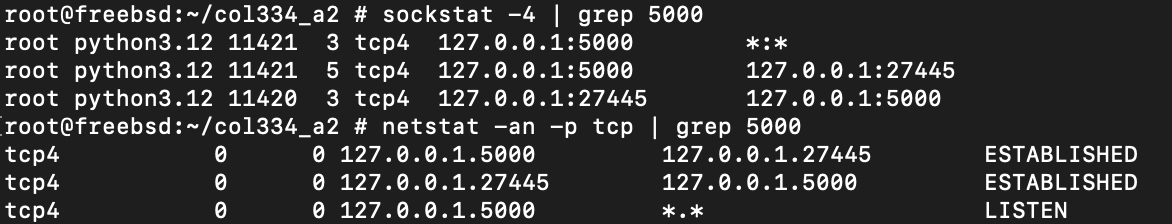
\includegraphics{screenshots/1a.png}\\
\emph{Figure 1: \texttt{sockstat} and \texttt{netstat} outputs during
Experiment 1, displaying the listening descriptor alongside the
established client connection.}

\textbf{Kernel Socket Table Inspection:}

\begin{verbatim}
$ sockstat -4 | grep 5000
root python3.12 4898  3 tcp4  127.0.0.1:5000        *:*
root python3.12 4898  5 tcp4  127.0.0.1:5000        127.0.0.1:28907
root python3.12 4897  3 tcp4  127.0.0.1:28907       127.0.0.1:5000

$ netstat -an -p tcp | grep 5000
tcp4  0  0  127.0.0.1.5000    127.0.0.1.28907   ESTABLISHED
tcp4  0  0  127.0.0.1.28907   127.0.0.1.5000    ESTABLISHED
tcp4  0  0  127.0.0.1.5000    *.*               LISTEN
\end{verbatim}

\textbf{Table 1: Exchange Server Socket Descriptors}

\begin{longtable}[]{@{}
  >{\raggedright\arraybackslash}p{(\columnwidth - 8\tabcolsep) * \real{0.2000}}
  >{\raggedright\arraybackslash}p{(\columnwidth - 8\tabcolsep) * \real{0.2000}}
  >{\raggedright\arraybackslash}p{(\columnwidth - 8\tabcolsep) * \real{0.2000}}
  >{\raggedright\arraybackslash}p{(\columnwidth - 8\tabcolsep) * \real{0.2000}}
  >{\raggedright\arraybackslash}p{(\columnwidth - 8\tabcolsep) * \real{0.2000}}@{}}
\toprule\noalign{}
\begin{minipage}[b]{\linewidth}\raggedright
File Descriptor
\end{minipage} & \begin{minipage}[b]{\linewidth}\raggedright
Socket Role
\end{minipage} & \begin{minipage}[b]{\linewidth}\raggedright
Local Address
\end{minipage} & \begin{minipage}[b]{\linewidth}\raggedright
Foreign Address
\end{minipage} & \begin{minipage}[b]{\linewidth}\raggedright
TCP State
\end{minipage} \\
\midrule\noalign{}
\endhead
\bottomrule\noalign{}
\endlastfoot
\texttt{fd=3} & Listening Acceptor & \texttt{127.0.0.1:5000} &
\texttt{*:*} & \texttt{LISTEN} \\
\texttt{fd=5} (\texttt{sid=2}) & Active Connection &
\texttt{127.0.0.1:5000} & \texttt{127.0.0.1:28907} &
\texttt{ESTABLISHED} \\
\end{longtable}

\begin{center}\rule{0.5\linewidth}{0.5pt}\end{center}

\hypertarget{experiment-2-observing-tcp-connection-states}{%
\subsection{3. Experiment 2 --- Observing TCP Connection
States}\label{experiment-2-observing-tcp-connection-states}}

\hypertarget{technical-analysis-1}{%
\subsubsection{3.1 Technical Analysis}\label{technical-analysis-1}}

TCP connection lifecycles follow a strict state progression:

\begin{enumerate}
\def\labelenumi{\arabic{enumi}.}
\tightlist
\item
  \textbf{Connection Setup:} The three-way handshake transitions
  endpoints from \texttt{LISTEN} / \texttt{SYN\_SENT} \(\to\)
  \texttt{SYN\_RECEIVED} \(\to\) \texttt{ESTABLISHED}.
\item
  \textbf{Orderly Teardown:} The client acts as the active closer by
  invoking \texttt{close()}, transmitting a \texttt{FIN} control
  segment. The client enters \texttt{FIN\_WAIT\_1}, while the server
  transitions to \texttt{CLOSE\_WAIT} upon acknowledging the
  \texttt{FIN}.
\item
  \textbf{Server Completion:} The server reads EOF (\texttt{recv()}
  returning \texttt{b\textquotesingle{}\textquotesingle{}}), closes its
  local descriptor, and sends its own \texttt{FIN}, transitioning to
  \texttt{LAST\_ACK}.
\item
  \textbf{Final Closure:} Upon receiving the server's \texttt{FIN}, the
  client sends a final \texttt{ACK} and enters \texttt{TIME\_WAIT}
  (retained for \(2\times\text{MSL}\) to absorb delayed duplicate
  segments), while the server transitions directly to \texttt{CLOSED}.
\end{enumerate}

Because our event loop promptly detects EOF on read readiness, the
server's duration in \texttt{CLOSE\_WAIT} is minimal (measured between
\(504\,\mu\text{s}\) and \(984\,\mu\text{s}\)), completely preventing
file descriptor exhaustion.

\hypertarget{investigation-methodology-tools-1}{%
\subsubsection{3.2 Investigation Methodology \&
Tools}\label{investigation-methodology-tools-1}}

Full packet capture on \texttt{lo0} combined with high-frequency
\texttt{netstat} sampling:

\begin{Shaded}
\begin{Highlighting}[]
\ExtensionTok{tcpdump} \AttributeTok{{-}i}\NormalTok{ lo0 }\AttributeTok{{-}n} \AttributeTok{{-}s0} \AttributeTok{{-}w}\NormalTok{ exp2.pcap }\StringTok{\textquotesingle{}tcp port 5000\textquotesingle{}} \KeywordTok{\&}
\ExtensionTok{python3}\NormalTok{ experiment.py 2}
\FunctionTok{netstat} \AttributeTok{{-}an} \AttributeTok{{-}p}\NormalTok{ tcp }\KeywordTok{|} \FunctionTok{grep}\NormalTok{ 5000}
\ExtensionTok{tcpdump} \AttributeTok{{-}r}\NormalTok{ exp2.pcap }\AttributeTok{{-}n} \AttributeTok{{-}ttt} \AttributeTok{{-}S}
\end{Highlighting}
\end{Shaded}

\hypertarget{empirical-evidence-1}{%
\subsubsection{3.3 Empirical Evidence}\label{empirical-evidence-1}}

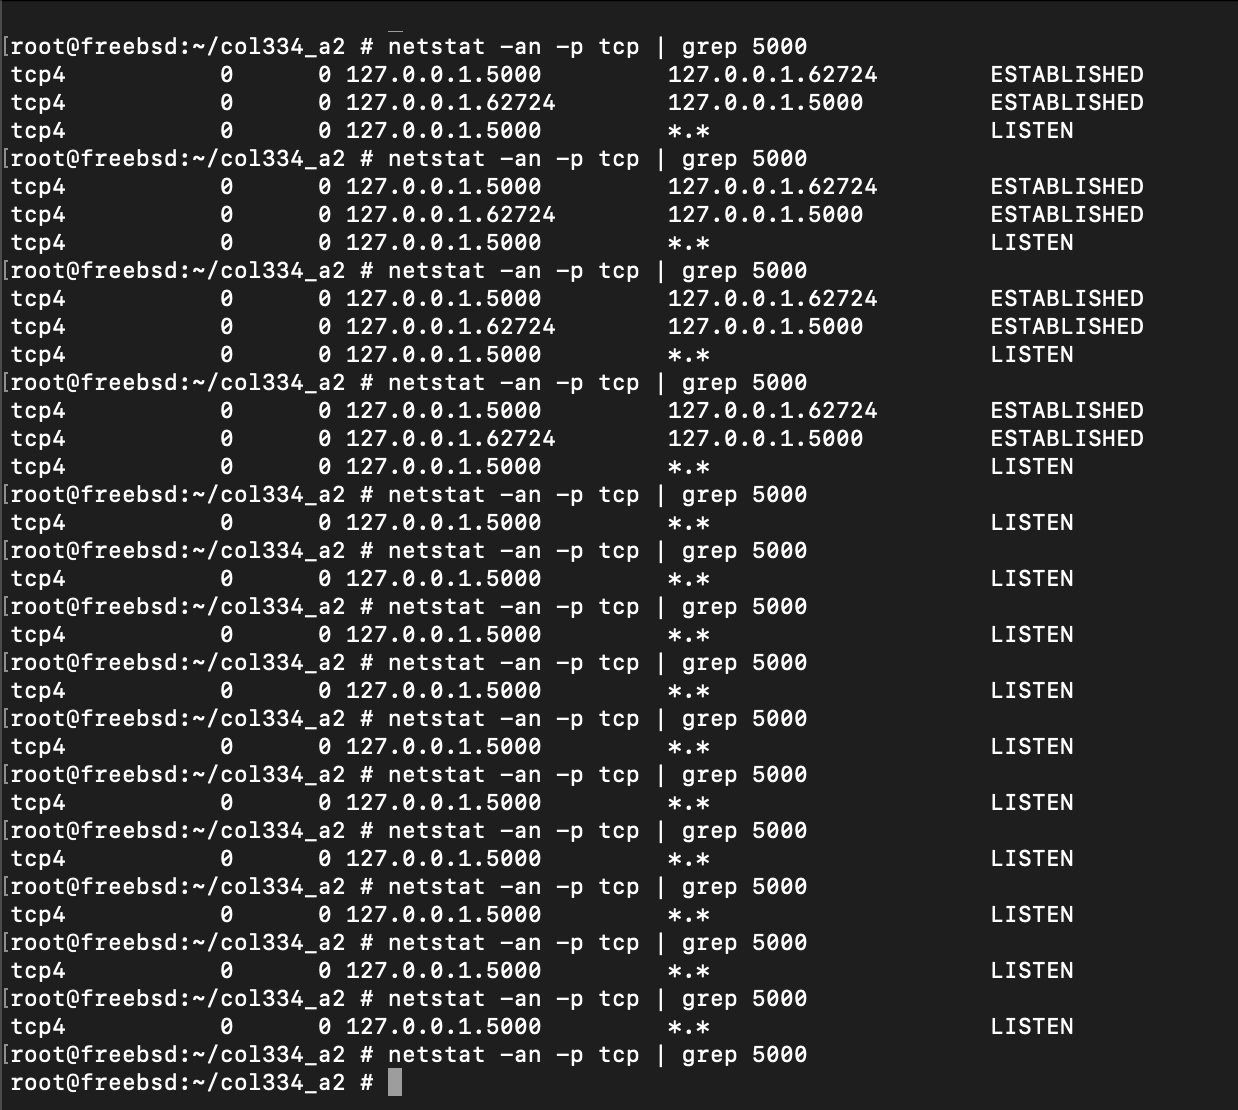
\includegraphics{screenshots/2a.png}\\
\emph{Figure 2a: Repeated \texttt{netstat} sampling across connection
and disconnection phases.}

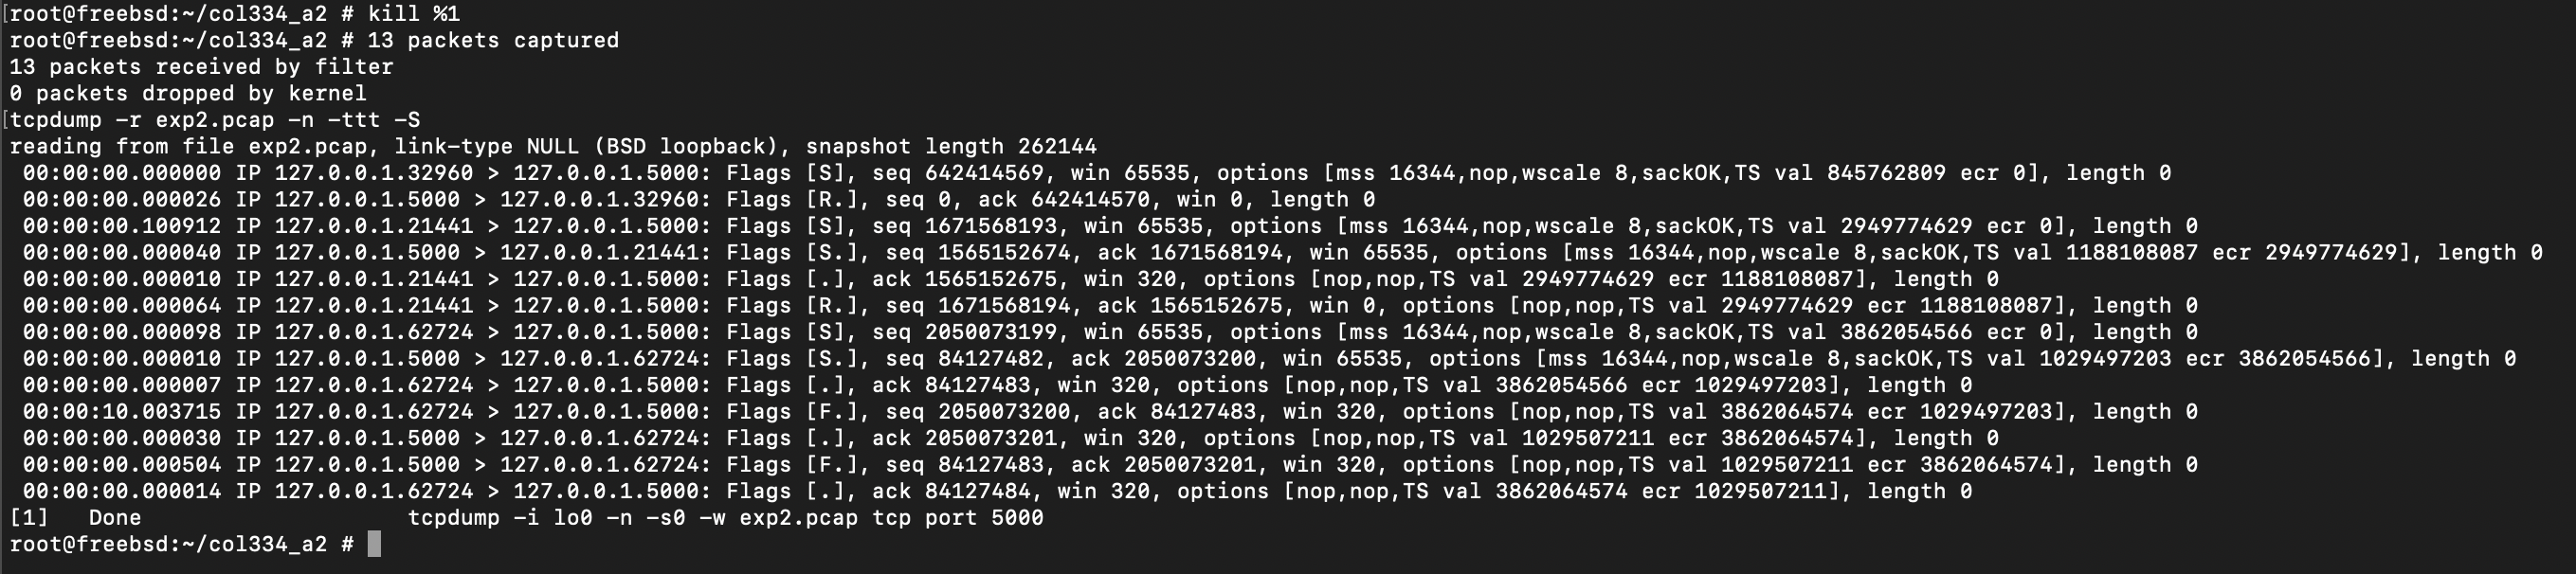
\includegraphics{screenshots/2b.png}\\
\emph{Figure 2b: Wire-level packet capture confirming the complete
four-way handshake and teardown.}

\textbf{Packet Trace Chronology (\texttt{exp2.pcap}):}

\begin{verbatim}
+0.000098s  SYN 62724->5000 -> SYN/ACK -> ACK       (Handshake established)
+10.003715s [62724->5000] FIN,ACK                  (Client initiates close)
+0.000030s  [5000->62724] ACK                      (Server ACKs; enters CLOSE_WAIT)
+0.000504s  [5000->62724] FIN,ACK                  (Server closes; enters LAST_ACK)
+0.000014s  [62724->5000] ACK                      (Client ACKs; enters TIME_WAIT)
\end{verbatim}

\textbf{Table 2: State Machine Transition Timeline}

\begin{longtable}[]{@{}
  >{\raggedright\arraybackslash}p{(\columnwidth - 6\tabcolsep) * \real{0.2500}}
  >{\raggedright\arraybackslash}p{(\columnwidth - 6\tabcolsep) * \real{0.2500}}
  >{\raggedright\arraybackslash}p{(\columnwidth - 6\tabcolsep) * \real{0.2500}}
  >{\raggedright\arraybackslash}p{(\columnwidth - 6\tabcolsep) * \real{0.2500}}@{}}
\toprule\noalign{}
\begin{minipage}[b]{\linewidth}\raggedright
Elapsed
\end{minipage} & \begin{minipage}[b]{\linewidth}\raggedright
Wire Event
\end{minipage} & \begin{minipage}[b]{\linewidth}\raggedright
Client State
\end{minipage} & \begin{minipage}[b]{\linewidth}\raggedright
Server State
\end{minipage} \\
\midrule\noalign{}
\endhead
\bottomrule\noalign{}
\endlastfoot
\(t_0\) & Handshake complete (\texttt{SYN} \(\to\) \texttt{SYN/ACK}
\(\to\) \texttt{ACK}) & \texttt{ESTABLISHED} & \texttt{ESTABLISHED} \\
\(t_0 + 10.0\,\text{s}\) & Client issues \texttt{close()}, sends
\texttt{FIN} & \texttt{FIN\_WAIT\_1} \(\to\) \texttt{FIN\_WAIT\_2} &
\texttt{CLOSE\_WAIT} \\
\(+30\,\mu\text{s}\) & Server acknowledges client \texttt{FIN} &
\texttt{FIN\_WAIT\_2} & \texttt{CLOSE\_WAIT} \\
\(+504\,\mu\text{s}\) & Server issues \texttt{close()}, sends
\texttt{FIN} & \texttt{TIME\_WAIT} & \texttt{LAST\_ACK} \\
\(+14\,\mu\text{s}\) & Client acknowledges server \texttt{FIN} &
\texttt{TIME\_WAIT} & \texttt{CLOSED} \\
\end{longtable}

\begin{center}\rule{0.5\linewidth}{0.5pt}\end{center}

\hypertarget{experiment-3-tcp-as-a-byte-stream}{%
\subsection{4. Experiment 3 --- TCP as a Byte
Stream}\label{experiment-3-tcp-as-a-byte-stream}}

\hypertarget{technical-analysis-2}{%
\subsubsection{4.1 Technical Analysis}\label{technical-analysis-2}}

TCP provides a structured byte stream service without preserving
application-level message boundaries. Network boundaries are determined
by sender buffering, MTU limits, TCP segment sizing, and transmission
timing. Application protocols running over TCP must implement explicit
framing.

In this experiment, the client transmits
\texttt{LOGIN\ experiment\_trader\textbackslash{}n} across four separate
\texttt{send()} operations spaced by 200 ms. The server performs four
discrete \texttt{recv()} invocations. The application framer buffers
incoming bytes until the \texttt{\textbackslash{}n} delimiter is
encountered, emitting the parsed command only upon receiving the fourth
segment.

\hypertarget{investigation-methodology-tools-2}{%
\subsubsection{4.2 Investigation Methodology \&
Tools}\label{investigation-methodology-tools-2}}

\begin{Shaded}
\begin{Highlighting}[]
\ExtensionTok{tcpdump} \AttributeTok{{-}i}\NormalTok{ lo0 }\AttributeTok{{-}n} \AttributeTok{{-}s0} \AttributeTok{{-}w}\NormalTok{ exp3.pcap }\StringTok{\textquotesingle{}tcp port 5000\textquotesingle{}} \KeywordTok{\&}
\ExtensionTok{python3}\NormalTok{ experiment.py 3}
\ExtensionTok{tcpdump} \AttributeTok{{-}r}\NormalTok{ exp3.pcap }\AttributeTok{{-}n} \AttributeTok{{-}ttt} \AttributeTok{{-}S}
\end{Highlighting}
\end{Shaded}

\hypertarget{empirical-evidence-2}{%
\subsubsection{4.3 Empirical Evidence}\label{empirical-evidence-2}}

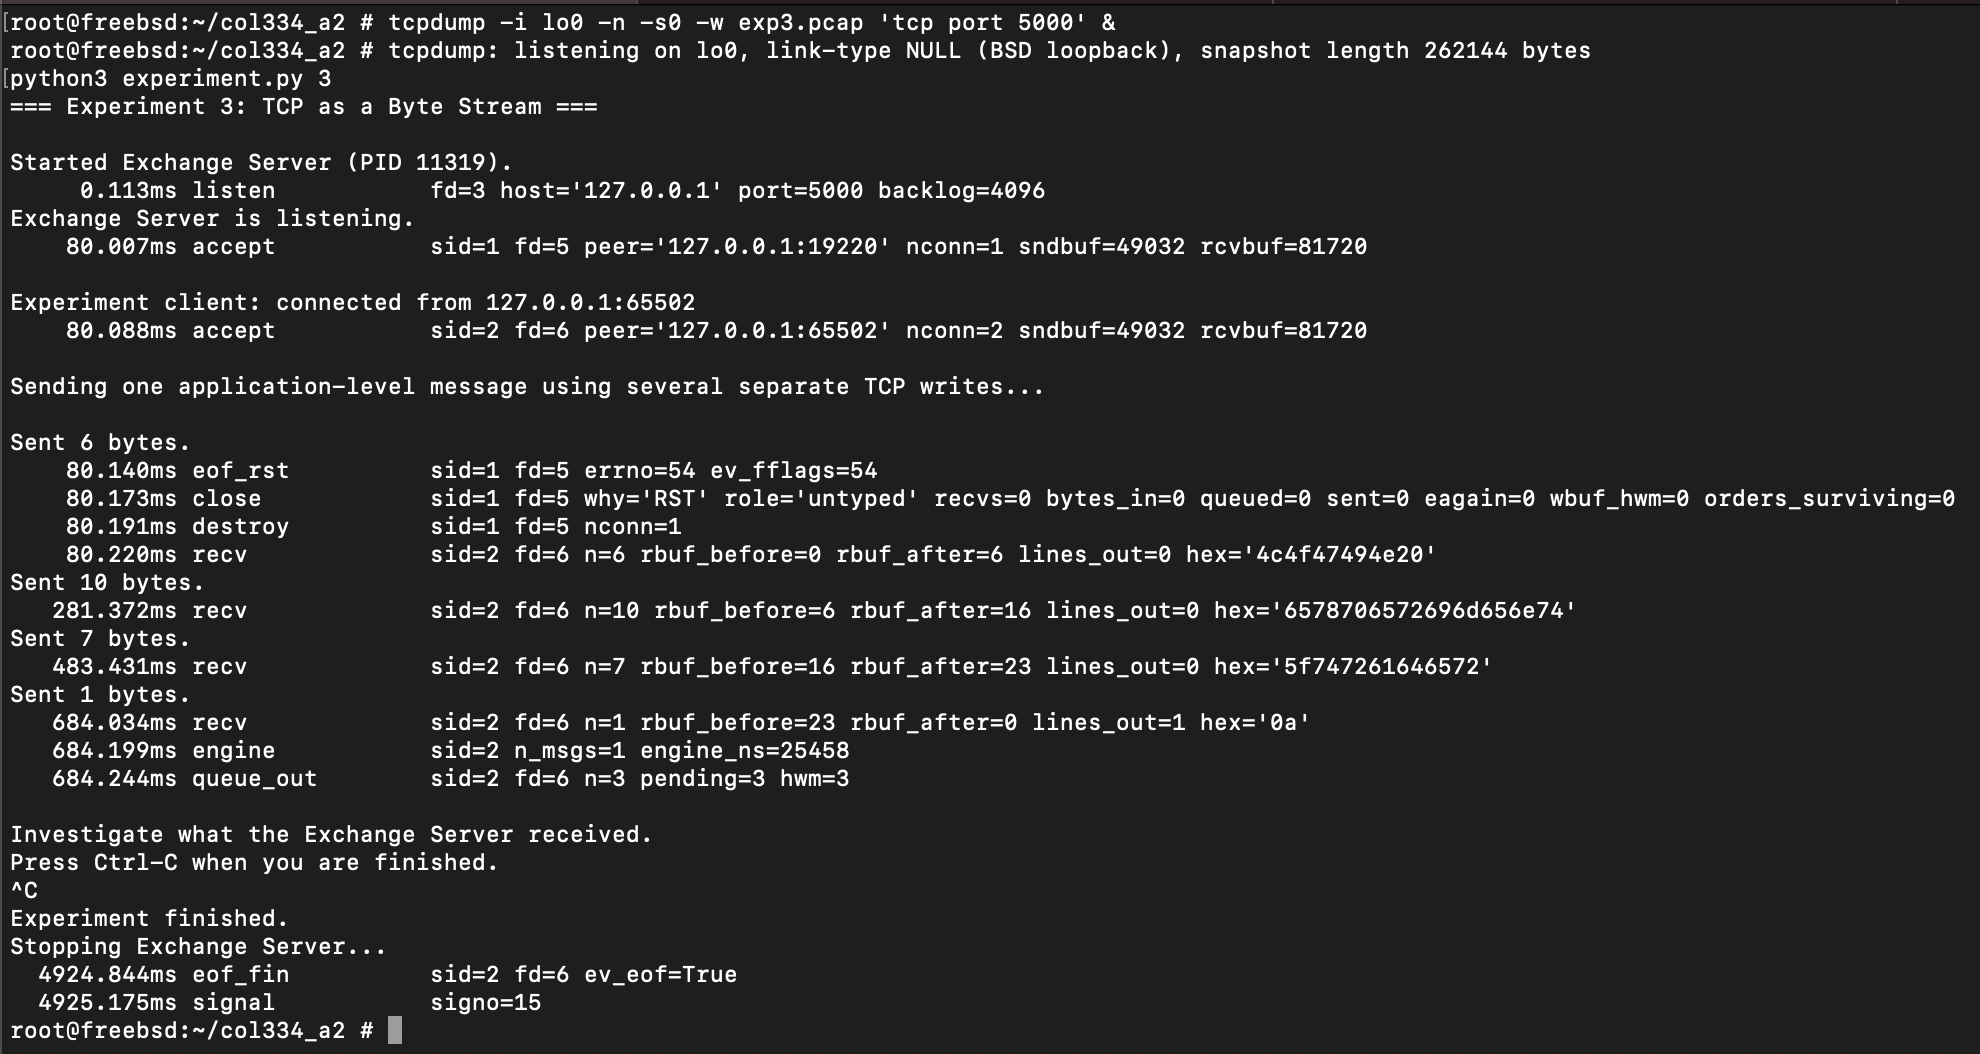
\includegraphics{screenshots/3a.png}\\
\emph{Figure 3a: Server execution trace detailing partial reads, buffer
accumulation, and final dispatch.}

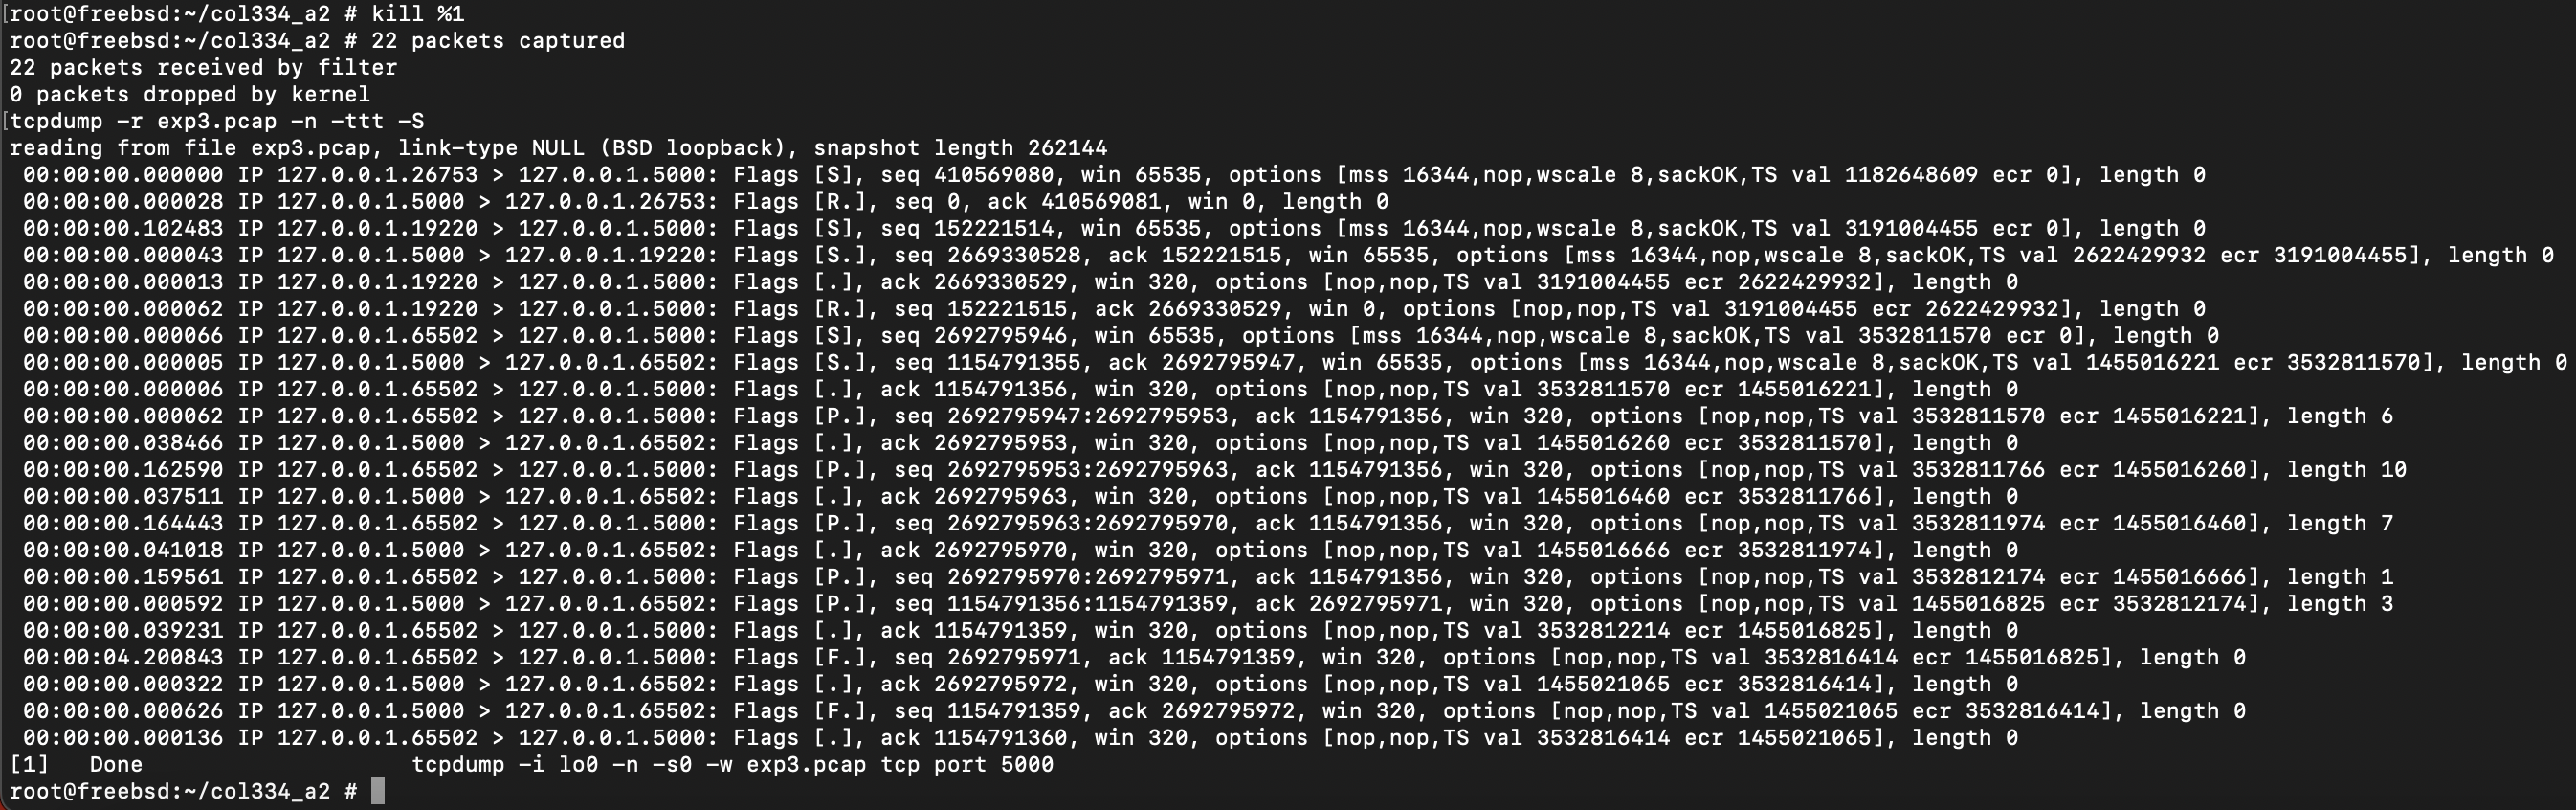
\includegraphics{screenshots/3b.png}\\
\emph{Figure 3b: Packet readback confirming four distinct PSH segments
arriving over loopback.}

\textbf{Server Trace Analysis:}

\begin{verbatim}
Time      Event sid fd n  rbuf_pre rbuf_post lines Payload
80.220ms  recv  2   6  6  0        6         0     "LOGIN "
281.372ms recv  2   6  10 6        16        0     "experiment"
483.431ms recv  2   6  7  16       23        0     "_trader"
684.034ms recv  2   6  1  23       0         1     "\n"
684.199ms engine dispatch: sid=2, messages=1, latency=25.4 us
\end{verbatim}

\textbf{Table 3: Stream Reassembly Ledger}

\begin{longtable}[]{@{}
  >{\centering\arraybackslash}p{(\columnwidth - 8\tabcolsep) * \real{0.2000}}
  >{\centering\arraybackslash}p{(\columnwidth - 8\tabcolsep) * \real{0.2000}}
  >{\centering\arraybackslash}p{(\columnwidth - 8\tabcolsep) * \real{0.2000}}
  >{\centering\arraybackslash}p{(\columnwidth - 8\tabcolsep) * \real{0.2000}}
  >{\centering\arraybackslash}p{(\columnwidth - 8\tabcolsep) * \real{0.2000}}@{}}
\toprule\noalign{}
\begin{minipage}[b]{\linewidth}\centering
Chunk
\end{minipage} & \begin{minipage}[b]{\linewidth}\centering
Interval
\end{minipage} & \begin{minipage}[b]{\linewidth}\centering
Length
\end{minipage} & \begin{minipage}[b]{\linewidth}\centering
Cumulative Buffer
\end{minipage} & \begin{minipage}[b]{\linewidth}\centering
Parser Status
\end{minipage} \\
\midrule\noalign{}
\endhead
\bottomrule\noalign{}
\endlastfoot
1 & 80 ms & 6 B & \texttt{LOGIN} (6 B) & Incomplete (0 emitted) \\
2 & 281 ms & 10 B & \texttt{LOGIN\ experiment} (16 B) & Incomplete (0
emitted) \\
3 & 483 ms & 7 B & \texttt{LOGIN\ experiment\_trader} (23 B) &
Incomplete (0 emitted) \\
4 & 684 ms & 1 B & Frame complete on \texttt{\textbackslash{}n} &
Emitted 1 command (\texttt{OK} returned) \\
\end{longtable}

Offline unit tests in \texttt{tests/test\_all.py} further verify stream
reassembly invariance across all 47 possible 2-way split permutations
and 1,000 randomized multi-fragment cuts.

\begin{center}\rule{0.5\linewidth}{0.5pt}\end{center}

\hypertarget{experiment-4-one-client-should-not-stall-the-others}{%
\subsection{5. Experiment 4 --- One Client Should Not Stall the
Others}\label{experiment-4-one-client-should-not-stall-the-others}}

\hypertarget{technical-analysis-3}{%
\subsubsection{5.1 Technical Analysis}\label{technical-analysis-3}}

In an unmultiplexed, blocking architecture, a client that connects and
halts mid-message causes the server process or thread to block inside
\texttt{recv()}. The server becomes incapable of accepting new
connections or servicing other clients.

Using an event-driven kqueue architecture, the server waits exclusively
inside \texttt{kevent()}. A descriptor is only returned when the
operating system indicates read readiness. While Client 1 sits idle
without terminating its line, the server services Client 2
instantaneously (elapsed time: 0.003 s).

\hypertarget{comparative-investigation-ab-control}{%
\subsubsection{5.2 Comparative Investigation (A/B
Control)}\label{comparative-investigation-ab-control}}

To empirically verify the blocking mechanism, a baseline blocking server
(\texttt{src/naive\_server.py}) was evaluated under identical
conditions:

\begin{Shaded}
\begin{Highlighting}[]
\ExtensionTok{python3}\NormalTok{ experiment.py 4                       }\CommentTok{\# Production kqueue server}
\VariableTok{EXCH\_NAIVE}\OperatorTok{=}\NormalTok{1 }\ExtensionTok{python3}\NormalTok{ experiment.py 4          }\CommentTok{\# Blocking baseline control}
\FunctionTok{ps} \AttributeTok{{-}o}\NormalTok{ pid,tid,wchan,state }\AttributeTok{{-}p} \OperatorTok{\textless{}}\NormalTok{pid}\OperatorTok{\textgreater{}}
\end{Highlighting}
\end{Shaded}

\hypertarget{empirical-evidence-3}{%
\subsubsection{5.3 Empirical Evidence}\label{empirical-evidence-3}}

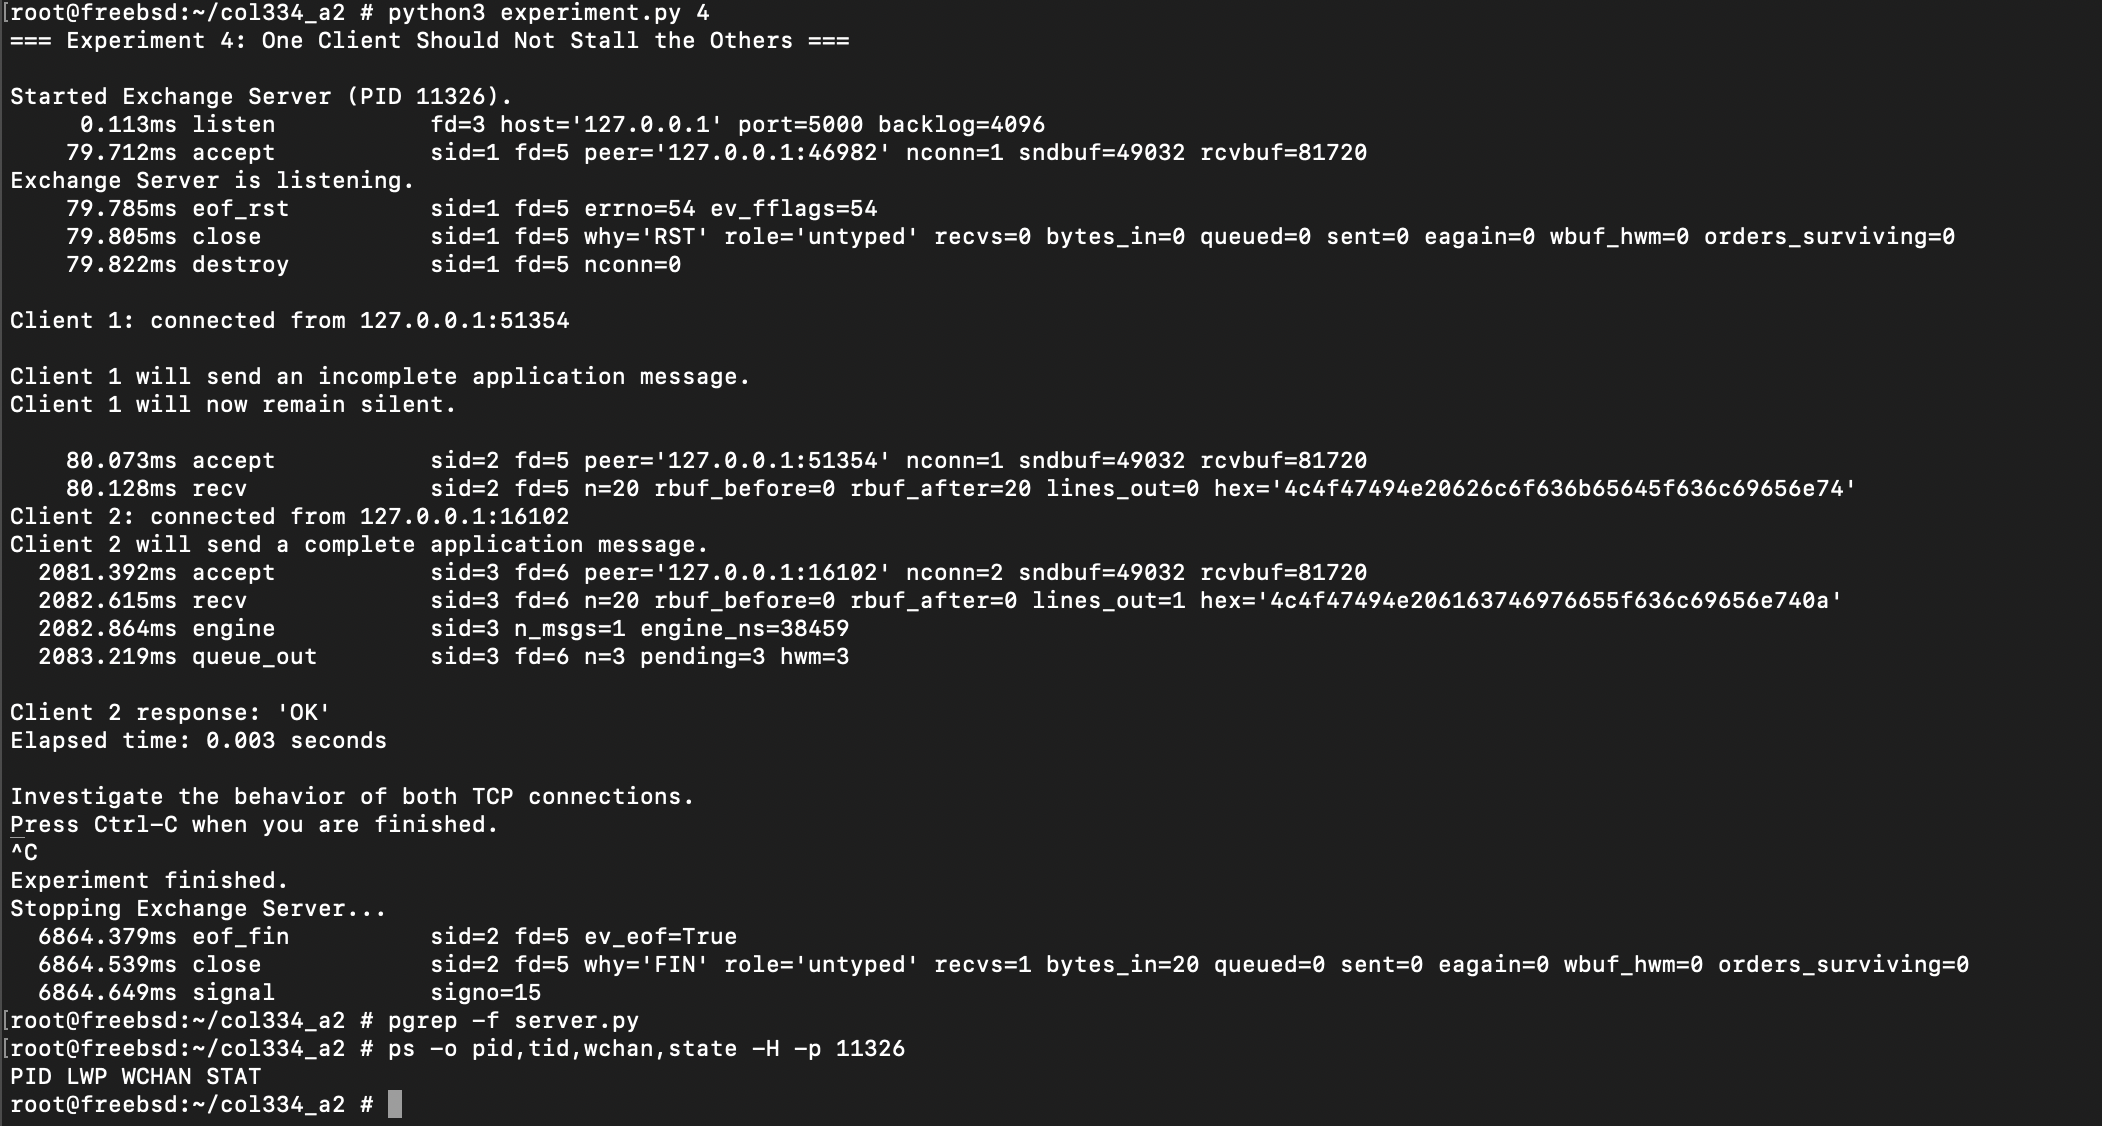
\includegraphics{screenshots/4a.png}\\
\emph{Figure 4a: Production server execution: Client 2 completes in
0.003 s with kernel wait channel \texttt{wchan=kqread}.}

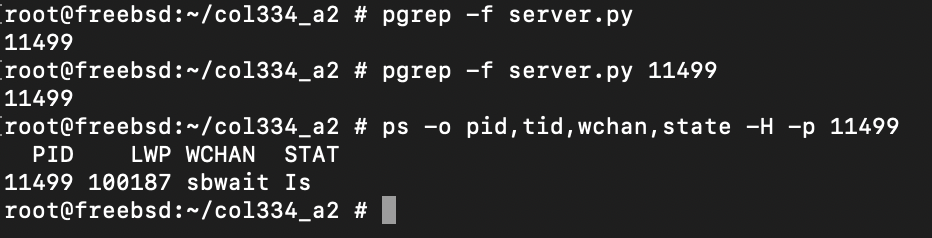
\includegraphics{screenshots/4b.png}\\
\emph{Figure 4b: Blocking baseline execution: Client 2 times out after
5.07 s with kernel wait channel \texttt{wchan=sbwait}.}

\textbf{Table 4: Concurrency Performance \& Wait Channel Comparison}

\begin{longtable}[]{@{}
  >{\raggedright\arraybackslash}p{(\columnwidth - 4\tabcolsep) * \real{0.3333}}
  >{\raggedright\arraybackslash}p{(\columnwidth - 4\tabcolsep) * \real{0.3333}}
  >{\raggedright\arraybackslash}p{(\columnwidth - 4\tabcolsep) * \real{0.3333}}@{}}
\toprule\noalign{}
\begin{minipage}[b]{\linewidth}\raggedright
Metric / Parameter
\end{minipage} & \begin{minipage}[b]{\linewidth}\raggedright
Production Server (\texttt{server.py})
\end{minipage} & \begin{minipage}[b]{\linewidth}\raggedright
Blocking Baseline (\texttt{naive\_server.py})
\end{minipage} \\
\midrule\noalign{}
\endhead
\bottomrule\noalign{}
\endlastfoot
\textbf{I/O Mechanism} & Non-blocking \texttt{select.kqueue()} &
Blocking POSIX sockets \\
\textbf{Kernel Wait Channel (\texttt{wchan})} & \textbf{\texttt{kqread}}
(waiting in \texttt{kevent}) & \textbf{\texttt{sbwait}} (blocked on
socket buffer read) \\
\textbf{Client 2 Response} & \texttt{OK} & \texttt{None} (Timed out) \\
\textbf{Client 2 Elapsed Time} & \textbf{0.003 s} & \textbf{5.072 s} \\
\textbf{Client 1 Socket Queue (\texttt{Recv-Q})} & \texttt{0} (Buffered
in userspace \texttt{rbuf}) & \texttt{0} (Held blocked in kernel
\texttt{recv}) \\
\end{longtable}

The wait channel confirms the root behavior: \texttt{sbwait} reflects
thread suspension on an individual socket buffer, whereas
\texttt{kqread} indicates scalable multiplexing over all registered
descriptors.

\begin{center}\rule{0.5\linewidth}{0.5pt}\end{center}

\hypertarget{experiment-5-multiple-clients-and-io-multiplexing}{%
\subsection{6. Experiment 5 --- Multiple Clients and I/O
Multiplexing}\label{experiment-5-multiple-clients-and-io-multiplexing}}

\hypertarget{technical-analysis-4}{%
\subsubsection{6.1 Technical Analysis}\label{technical-analysis-4}}

I/O multiplexing decouples connection presence from CPU servicing cost.
Across five concurrently established connections where only three submit
data (Clients 1, 3, 5), the event loop is dispatched exclusively for
descriptors possessing unread socket buffers. Idle connections consume
zero CPU time, exhibiting \(O(\text{ready})\) rather than
\(O(\text{registered})\) scaling.

\hypertarget{investigation-methodology-tools-3}{%
\subsubsection{6.2 Investigation Methodology \&
Tools}\label{investigation-methodology-tools-3}}

\begin{Shaded}
\begin{Highlighting}[]
\ExtensionTok{python3}\NormalTok{ experiment.py 5}
\FunctionTok{netstat} \AttributeTok{{-}an} \AttributeTok{{-}p}\NormalTok{ tcp }\KeywordTok{|} \FunctionTok{grep} \StringTok{\textquotesingle{}\textbackslash{}.5000 \textquotesingle{}}
\end{Highlighting}
\end{Shaded}

\hypertarget{empirical-evidence-4}{%
\subsubsection{6.3 Empirical Evidence}\label{empirical-evidence-4}}

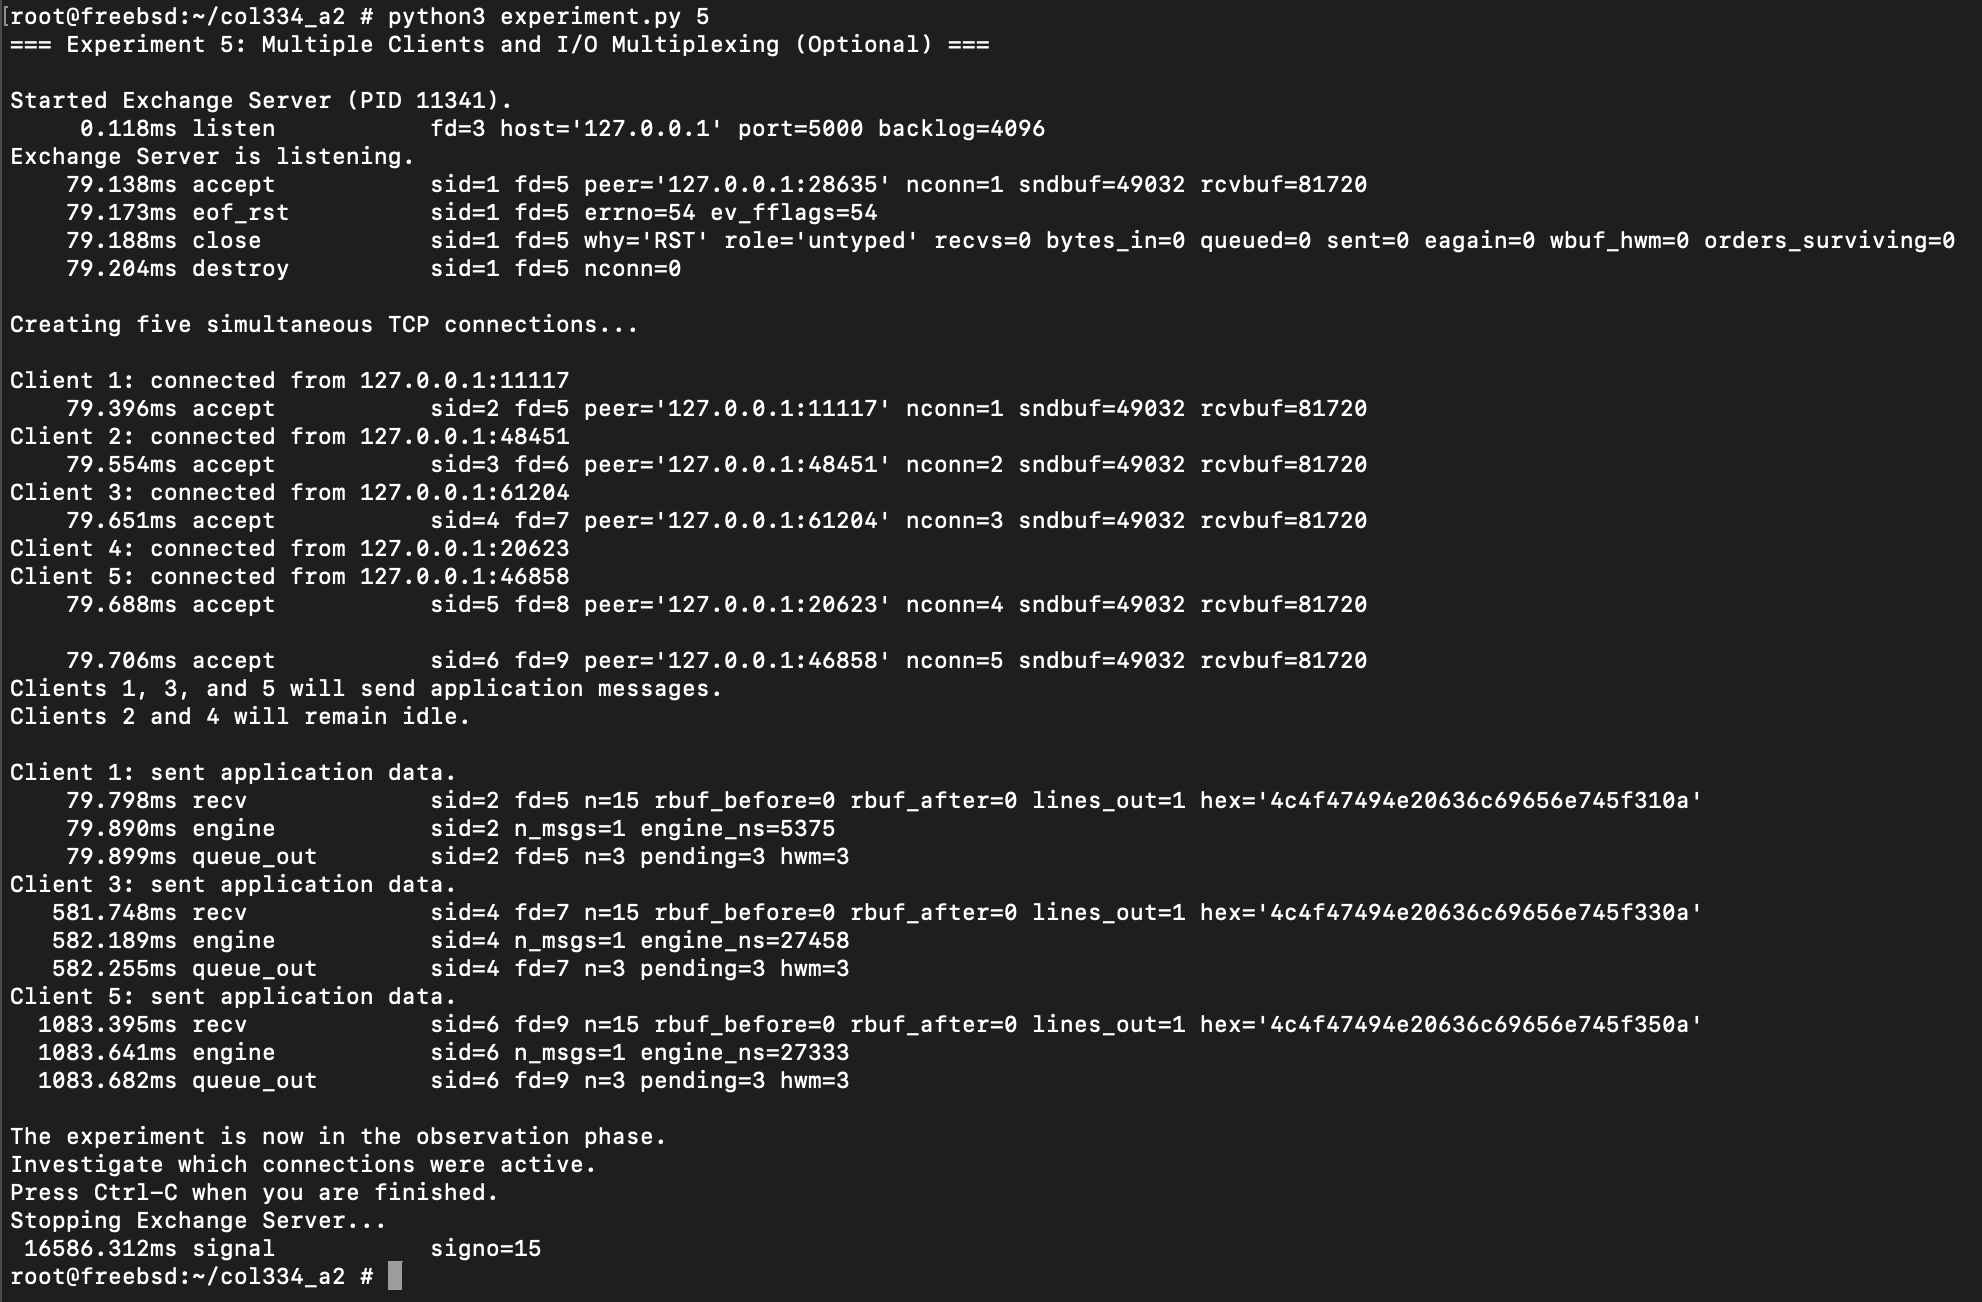
\includegraphics{screenshots/5a.png}\\
\emph{Figure 5a: Event loop execution trace confirming read events
trigger solely for active clients.}

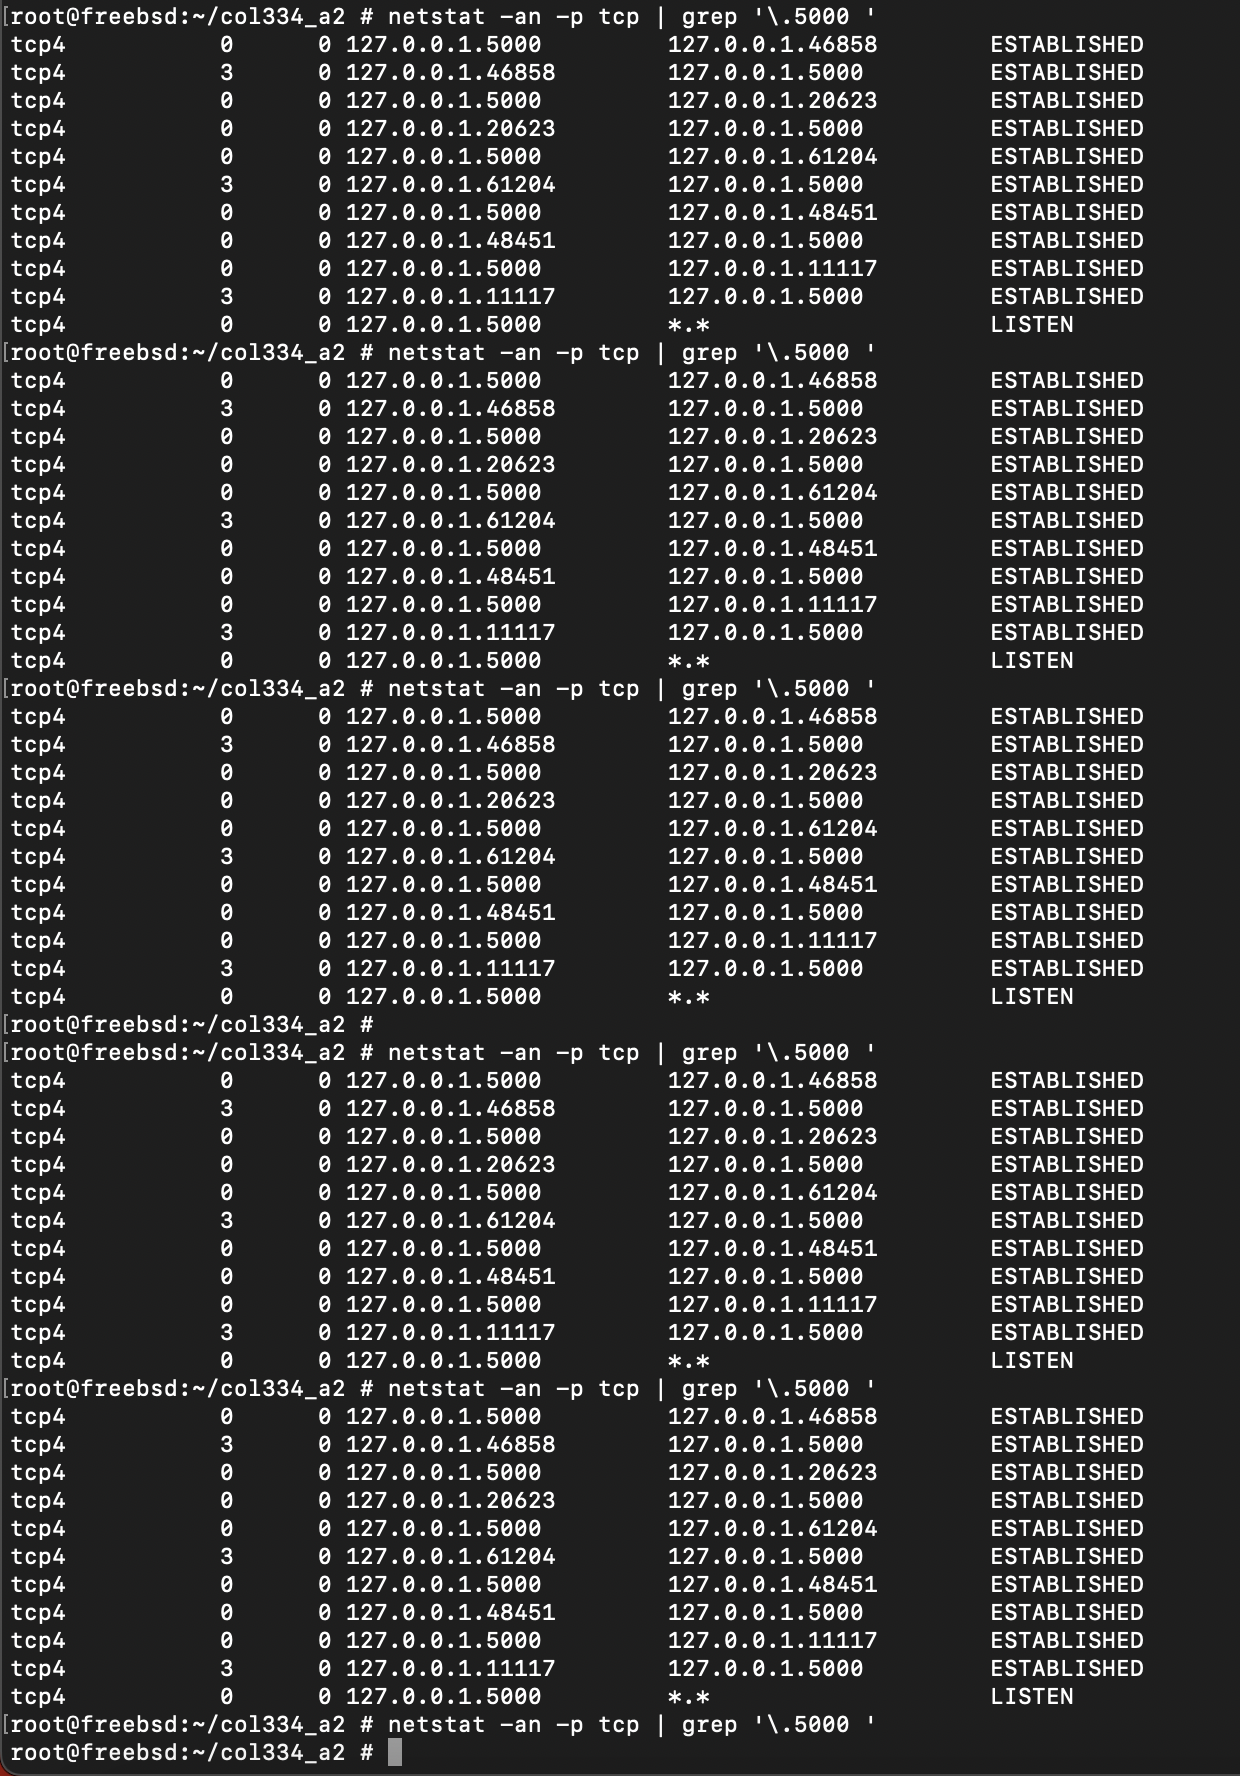
\includegraphics{screenshots/5b.png}\\
\emph{Figure 5b: System connection table showing all five connections
concurrently established.}

\textbf{Table 5: Connection Readiness vs.~Service Activity}

\begin{longtable}[]{@{}
  >{\centering\arraybackslash}p{(\columnwidth - 10\tabcolsep) * \real{0.1667}}
  >{\centering\arraybackslash}p{(\columnwidth - 10\tabcolsep) * \real{0.1667}}
  >{\centering\arraybackslash}p{(\columnwidth - 10\tabcolsep) * \real{0.1667}}
  >{\centering\arraybackslash}p{(\columnwidth - 10\tabcolsep) * \real{0.1667}}
  >{\centering\arraybackslash}p{(\columnwidth - 10\tabcolsep) * \real{0.1667}}
  >{\centering\arraybackslash}p{(\columnwidth - 10\tabcolsep) * \real{0.1667}}@{}}
\toprule\noalign{}
\begin{minipage}[b]{\linewidth}\centering
Session ID
\end{minipage} & \begin{minipage}[b]{\linewidth}\centering
File Descriptor
\end{minipage} & \begin{minipage}[b]{\linewidth}\centering
Foreign Port
\end{minipage} & \begin{minipage}[b]{\linewidth}\centering
Client Role
\end{minipage} & \begin{minipage}[b]{\linewidth}\centering
\texttt{recv()} Activity
\end{minipage} & \begin{minipage}[b]{\linewidth}\centering
\texttt{Recv-Q} Status
\end{minipage} \\
\midrule\noalign{}
\endhead
\bottomrule\noalign{}
\endlastfoot
\texttt{sid=2} & \texttt{fd=5} & 11117 & Client 1 & Active (1 read,
\texttt{OK} sent) & 3 B (Client unread reply) \\
\texttt{sid=3} & \texttt{fd=6} & 48451 & Client 2 & \textbf{None (Idle)}
& \textbf{0 B / 0 B} \\
\texttt{sid=4} & \texttt{fd=7} & 61204 & Client 3 & Active (1 read,
\texttt{OK} sent) & 3 B (Client unread reply) \\
\texttt{sid=5} & \texttt{fd=8} & 20623 & Client 4 & \textbf{None (Idle)}
& \textbf{0 B / 0 B} \\
\texttt{sid=6} & \texttt{fd=9} & 46858 & Client 5 & Active (1 read,
\texttt{OK} sent) & 3 B (Client unread reply) \\
\end{longtable}

\begin{center}\rule{0.5\linewidth}{0.5pt}\end{center}

\hypertarget{experiment-6-fin-vs.-rst-orderly-and-abrupt-termination}{%
\subsection{7. Experiment 6 --- FIN vs.~RST: Orderly and Abrupt
Termination}\label{experiment-6-fin-vs.-rst-orderly-and-abrupt-termination}}

\hypertarget{technical-analysis-5}{%
\subsubsection{7.1 Technical Analysis}\label{technical-analysis-5}}

\begin{itemize}
\tightlist
\item
  \textbf{Orderly Termination (\texttt{FIN}):} A synchronized protocol
  event initiated via \texttt{shutdown(SHUT\_WR)} or \texttt{close()}.
  The \texttt{FIN} control segment carries an incremented sequence
  number, guarantees in-order delivery of preceding data, allows
  graceful half-close, and places the active closer in
  \texttt{TIME\_WAIT}. The peer application detects closure via EOF
  (\texttt{recv()} returns
  \texttt{b\textquotesingle{}\textquotesingle{}}).
\item
  \textbf{Abrupt Termination (\texttt{RST}):} An immediate connection
  abort initiated via \texttt{SO\_LINGER\{on=1,\ timeout=0\}} or process
  termination errors. The \texttt{RST} segment is unsequenced, discards
  queued network buffers in both directions, generates no
  \texttt{TIME\_WAIT} state, and immediately surfaces as
  \texttt{ECONNRESET} (errno 54).
\end{itemize}

Under FreeBSD \texttt{kqueue}, socket errors are delivered directly
within the event structure (\texttt{ev.fflags}), allowing discrimination
between normal EOF and an abortive reset before issuing \texttt{recv()}.

\hypertarget{investigation-methodology-tools-4}{%
\subsubsection{7.2 Investigation Methodology \&
Tools}\label{investigation-methodology-tools-4}}

\begin{Shaded}
\begin{Highlighting}[]
\ExtensionTok{tcpdump} \AttributeTok{{-}i}\NormalTok{ lo0 }\AttributeTok{{-}n} \AttributeTok{{-}s0} \AttributeTok{{-}w}\NormalTok{ exp6.pcap }\StringTok{\textquotesingle{}tcp port 5000\textquotesingle{}} \KeywordTok{\&}
\ExtensionTok{python3}\NormalTok{ experiment.py 6}
\ExtensionTok{tcpdump} \AttributeTok{{-}r}\NormalTok{ exp6.pcap }\AttributeTok{{-}n} \AttributeTok{{-}ttt} \AttributeTok{{-}S}
\end{Highlighting}
\end{Shaded}

\hypertarget{empirical-evidence-5}{%
\subsubsection{7.3 Empirical Evidence}\label{empirical-evidence-5}}

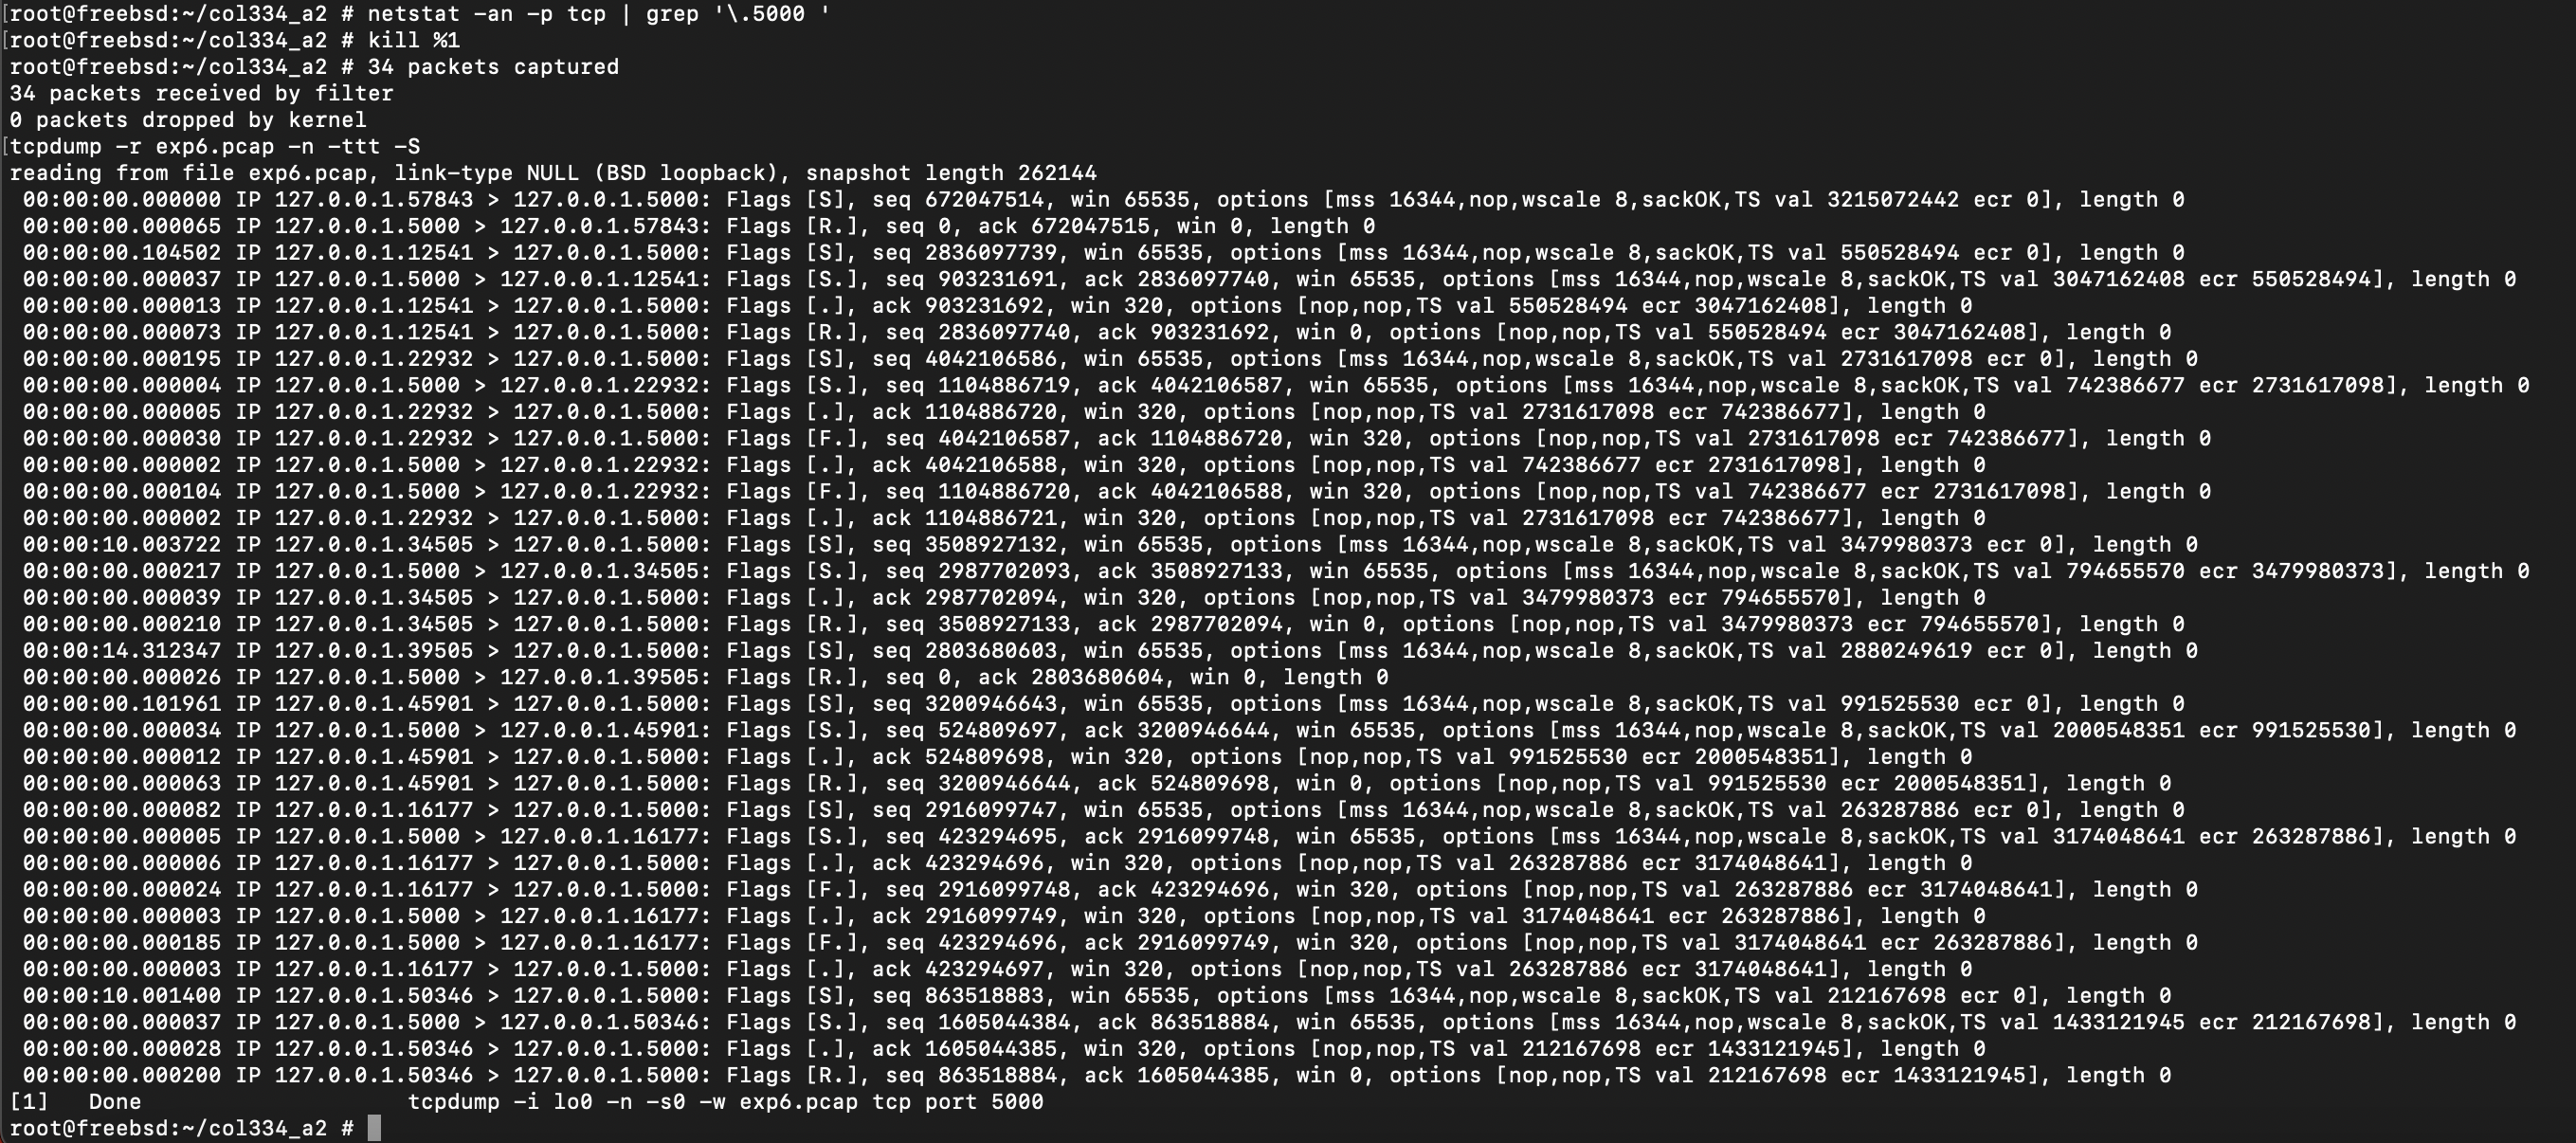
\includegraphics{screenshots/6a.png}\\
\emph{Figure 6a: Packet capture distinguishing four-way FIN handshake
(Part A) from single RST segment (Part B).}

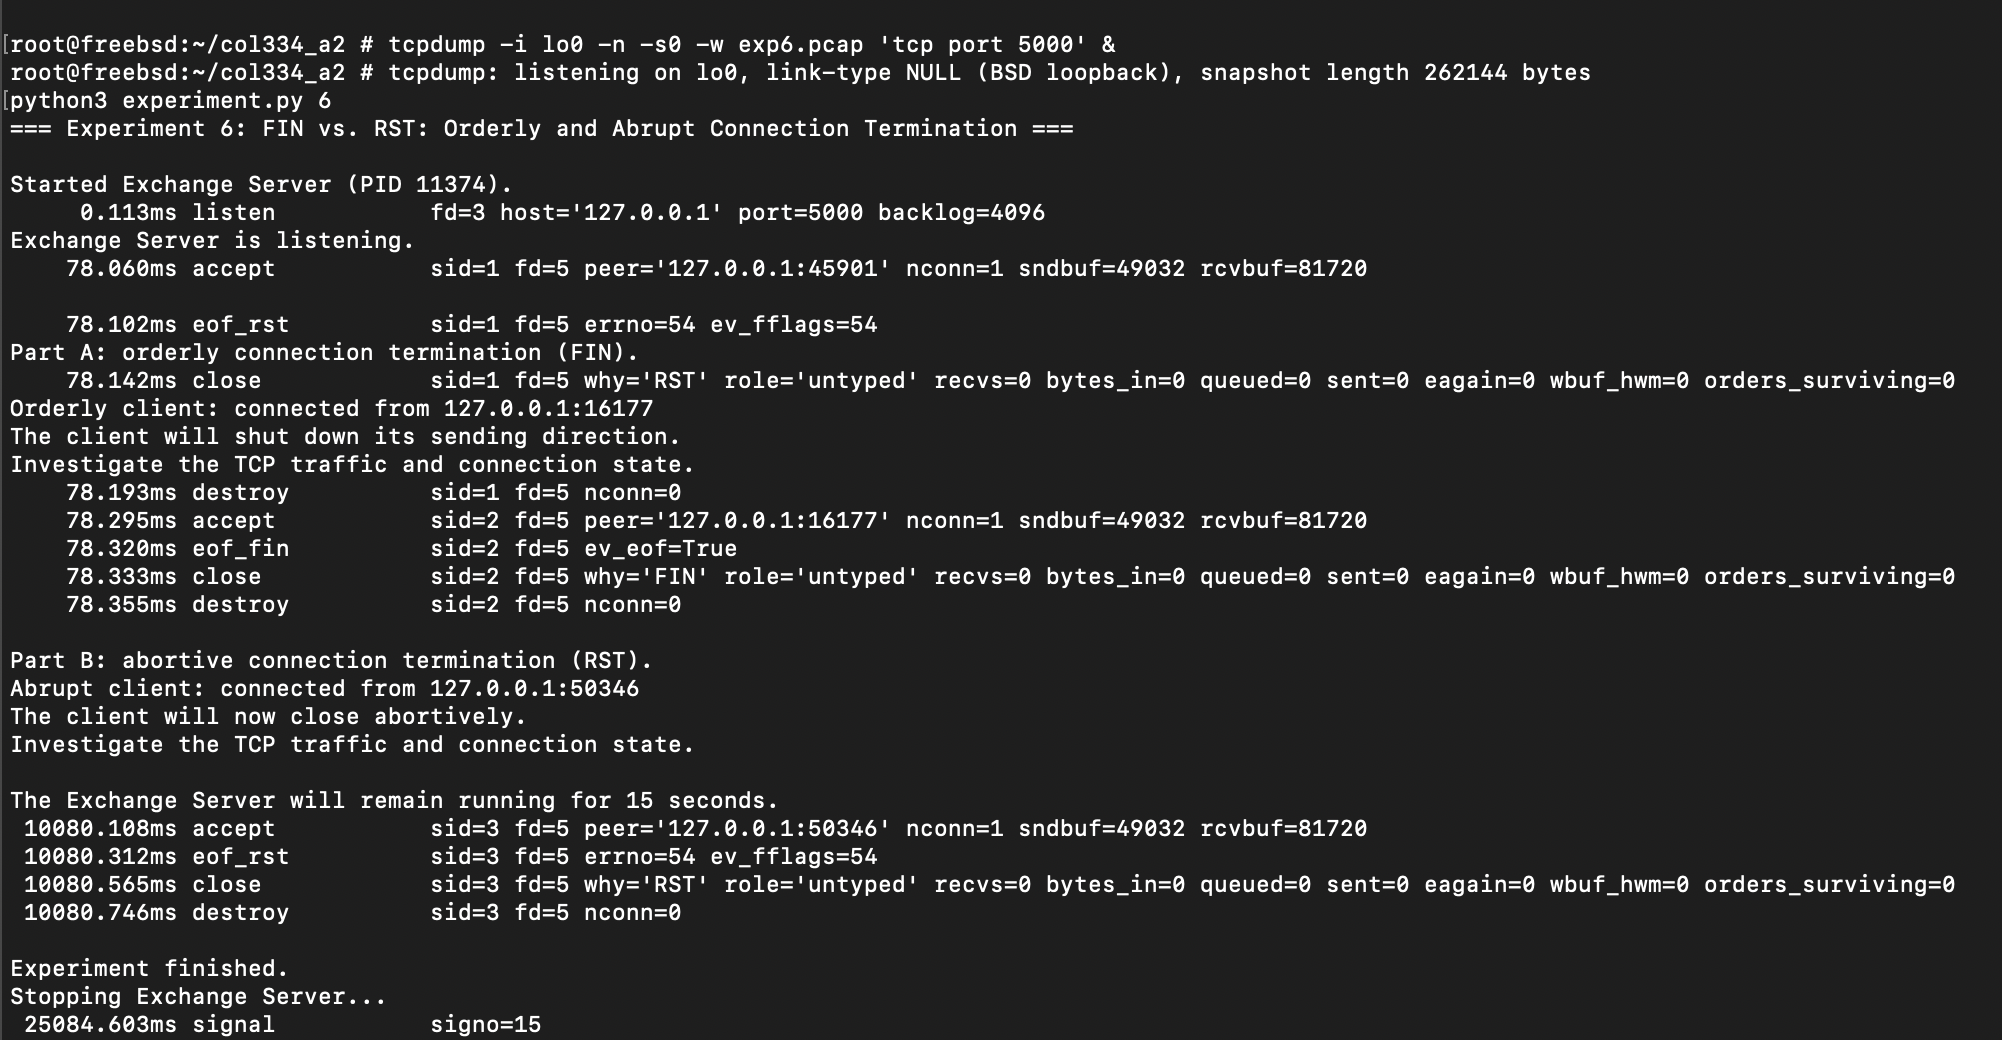
\includegraphics{screenshots/6b.png}\\
\emph{Figure 6b: Server logs detailing \texttt{eof\_fin} (Part A) versus
\texttt{eof\_rst} with errno 54 (Part B).}

\textbf{Wire Event Comparison:}

\begin{verbatim}
Part A (Orderly FIN - Port 16177):
  16177 > 5000: Flags [F.] seq 1 ack 1 (Client SHUT_WR)
  5000 > 16177: Flags [.]  ack 2        (Server ACK)
  5000 > 16177: Flags [F.] seq 1 ack 2 (Server FIN)
  16177 > 5000: Flags [.]  ack 2        (Client ACK)

Part B (Abrupt RST - Port 50346):
  50346 > 5000: Flags [R.] seq 1 win 0  (Immediate abortive reset)
\end{verbatim}

\textbf{Table 6: Teardown Mechanism Characteristics}

\begin{longtable}[]{@{}
  >{\raggedright\arraybackslash}p{(\columnwidth - 4\tabcolsep) * \real{0.3333}}
  >{\raggedright\arraybackslash}p{(\columnwidth - 4\tabcolsep) * \real{0.3333}}
  >{\raggedright\arraybackslash}p{(\columnwidth - 4\tabcolsep) * \real{0.3333}}@{}}
\toprule\noalign{}
\begin{minipage}[b]{\linewidth}\raggedright
Dimension
\end{minipage} & \begin{minipage}[b]{\linewidth}\raggedright
Orderly Termination (\texttt{FIN})
\end{minipage} & \begin{minipage}[b]{\linewidth}\raggedright
Abrupt Termination (\texttt{RST})
\end{minipage} \\
\midrule\noalign{}
\endhead
\bottomrule\noalign{}
\endlastfoot
\textbf{Packet Sequence} & 4-way exchange (\texttt{{[}F.{]}},
\texttt{{[}.{]}}, \texttt{{[}F.{]}}, \texttt{{[}.{]}}) & Single abortive
packet (\texttt{{[}R.{]}}) \\
\textbf{\texttt{recv()} Application Signal} & Returns empty bytes
(\texttt{b\textquotesingle{}\textquotesingle{}}) & Raises
\texttt{ConnectionResetError} \\
\textbf{FreeBSD Kernel Errno} & None (\(0\)) & \textbf{\(54\)
(\texttt{ECONNRESET})} \\
\textbf{Kqueue Event Notification} & \texttt{ev.flags\ \&\ KQ\_EV\_EOF}
& \texttt{ev.fflags\ ==\ 54} \\
\textbf{\texttt{TIME\_WAIT} State} & Enforced on active closer &
Completely bypassed \\
\textbf{Server State Effect} & Closed cleanly; surviving peers
unaffected & Closed cleanly; surviving peers unaffected \\
\end{longtable}

\begin{center}\rule{0.5\linewidth}{0.5pt}\end{center}

\hypertarget{experiment-7-backpressure-and-the-slow-receiver}{%
\subsection{8. Experiment 7 --- Backpressure and the Slow
Receiver}\label{experiment-7-backpressure-and-the-slow-receiver}}

\hypertarget{technical-analysis-theoretical-capacity}{%
\subsubsection{8.1 Technical Analysis \& Theoretical
Capacity}\label{technical-analysis-theoretical-capacity}}

When a subscriber ceases reading from its socket, incoming bytes
accumulate in its receive buffer. Once full, the receiver advertises a
zero-window (\texttt{win\ 0}), halting TCP transmissions. Continued
application write attempts then saturate the server's send buffer,
causing non-blocking \texttt{send()} calls to fail with
\texttt{EWOULDBLOCK} / \texttt{EAGAIN} (errno 35).

A properly decoupled server buffers excess messages in userspace and
registers write notification filters (\texttt{KQ\_FILTER\_WRITE}) for
the backlogged socket, ensuring other active clients and the core
matching engine continue operating uninhibited.

\hypertarget{initial-arithmetic-vs.-freebsd-loopback-behavior}{%
\subsubsection{8.2 Initial Arithmetic vs.~FreeBSD Loopback
Behavior}\label{initial-arithmetic-vs.-freebsd-loopback-behavior}}

In standard \texttt{experiment.py\ 7}:

\begin{itemize}
\tightlist
\item
  Message size: \texttt{TRADE\ JNST\ 1\ 238\textbackslash{}n} = 17
  bytes.
\item
  Order volume: 5,000 trade iterations = 85,003 bytes per subscriber
  (including 3 B \texttt{OK\textbackslash{}n}).
\item
  FreeBSD loopback socket buffers: default
  \texttt{sendspace\ =\ 32,768\ B}, \texttt{recvspace\ =\ 65,536\ B}
  (aggregate capacity \(\approx 98,304\text{ B}\)).
\end{itemize}

Because \(85,003 < 98,304\), the data fits entirely within kernel
buffers. Run A confirms this: \texttt{send\_would\_block\ =\ 0}, with
the slow subscriber's kernel \texttt{Recv-Q} absorbing all 83,232 bytes
while the active subscriber maintained \texttt{Recv-Q} near zero.

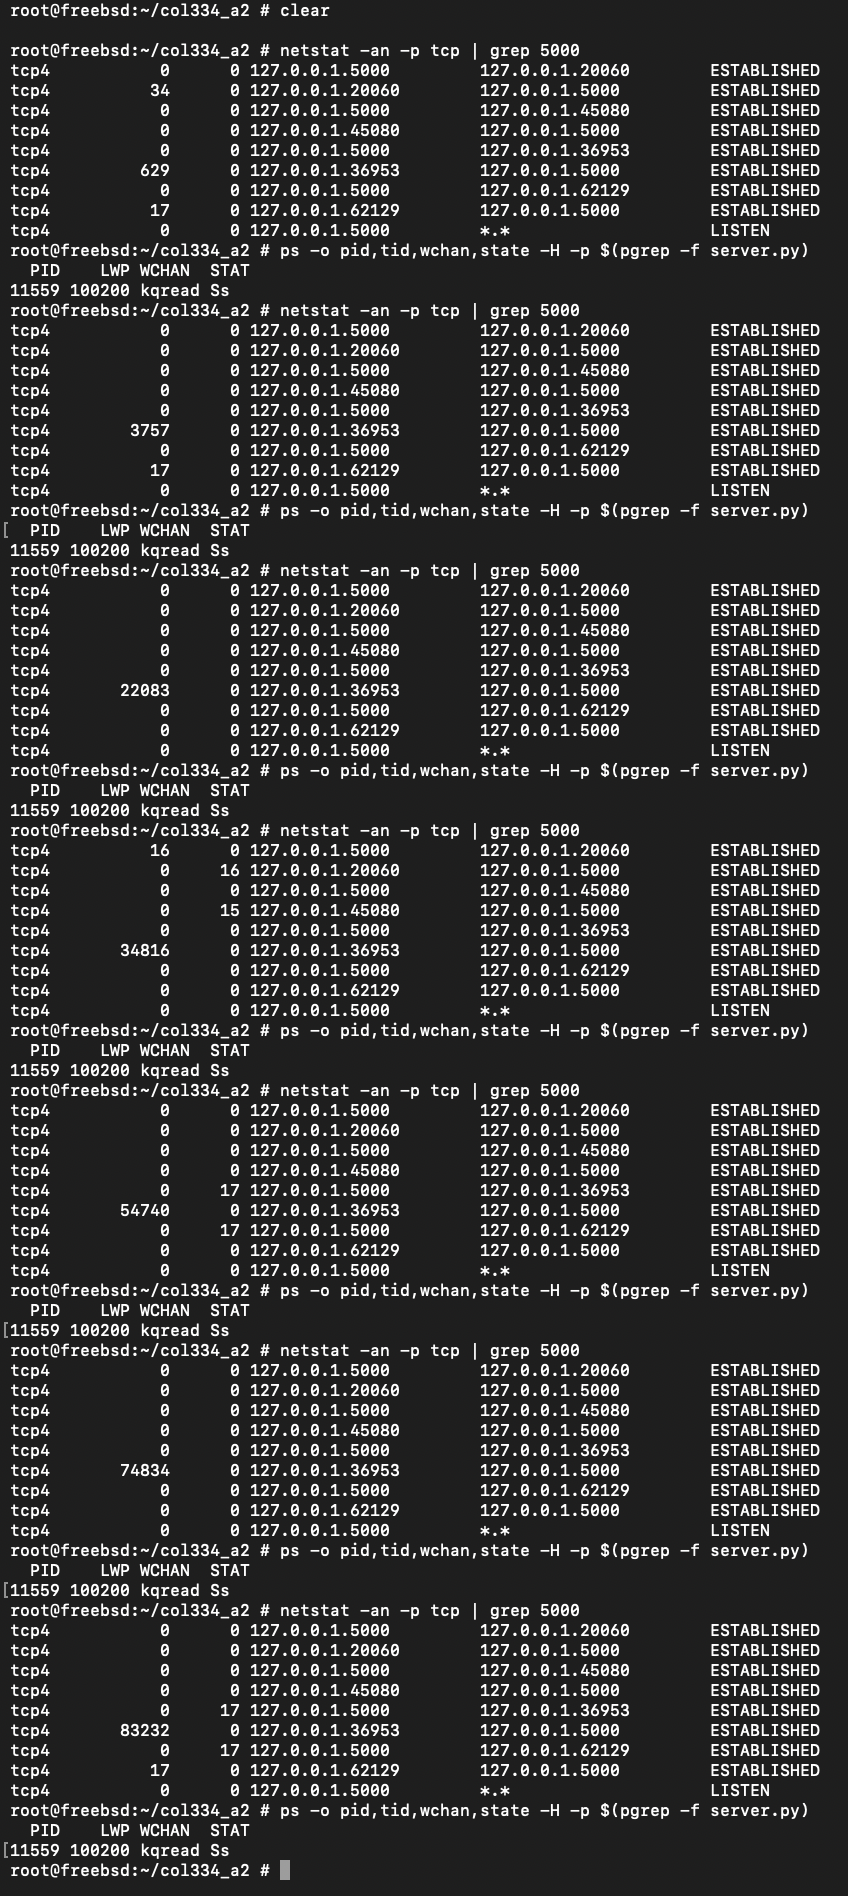
\includegraphics{screenshots/7a.png}\\
\emph{Figure 7a: \texttt{netstat} and \texttt{ps} sampling showing slow
subscriber \texttt{Recv-Q} scaling up to 83,232 B while server remains
in \texttt{kqread}.}

\textbf{Table 7: Run A Kernel Buffer Accumulation}

\begin{longtable}[]{@{}
  >{\centering\arraybackslash}p{(\columnwidth - 6\tabcolsep) * \real{0.2500}}
  >{\centering\arraybackslash}p{(\columnwidth - 6\tabcolsep) * \real{0.2500}}
  >{\centering\arraybackslash}p{(\columnwidth - 6\tabcolsep) * \real{0.2500}}
  >{\centering\arraybackslash}p{(\columnwidth - 6\tabcolsep) * \real{0.2500}}@{}}
\toprule\noalign{}
\begin{minipage}[b]{\linewidth}\centering
Sample
\end{minipage} & \begin{minipage}[b]{\linewidth}\centering
Fast Subscriber \texttt{Recv-Q}
\end{minipage} & \begin{minipage}[b]{\linewidth}\centering
Slow Subscriber \texttt{Recv-Q}
\end{minipage} & \begin{minipage}[b]{\linewidth}\centering
Server \texttt{wchan}
\end{minipage} \\
\midrule\noalign{}
\endhead
\bottomrule\noalign{}
\endlastfoot
1 & 17 B & 629 B & \texttt{kqread} \\
2 & 17 B & 3,757 B & \texttt{kqread} \\
3 & 0 B & 22,083 B & \texttt{kqread} \\
4 & 0 B & 34,816 B & \texttt{kqread} \\
5 & 17 B & 54,740 B & \texttt{kqread} \\
6 & 0 B & 74,834 B & \texttt{kqread} \\
7 & 17 B & \textbf{83,232 B} & \texttt{kqread} \\
\end{longtable}

\hypertarget{platform-investigation-freebsd-loopback-flow-control}{%
\subsubsection{8.3 Platform Investigation: FreeBSD Loopback Flow
Control}\label{platform-investigation-freebsd-loopback-flow-control}}

To induce backpressure within the default 5,000-message quota, buffer
sizes were restricted via \texttt{SO\_RCVBUF=8192} and
\texttt{SO\_SNDBUF=1024}. However, \texttt{Recv-Q} continued to climb
past limits without triggering backpressure.

An isolated standalone diagnostic (\texttt{src/tools/sb\_probe.py})
revealed that on FreeBSD's loopback interface (\texttt{lo0}), when a
receiving process never reads, the TCP stack allocates kernel mbuf
clusters rather than enforcing strict window clamping:

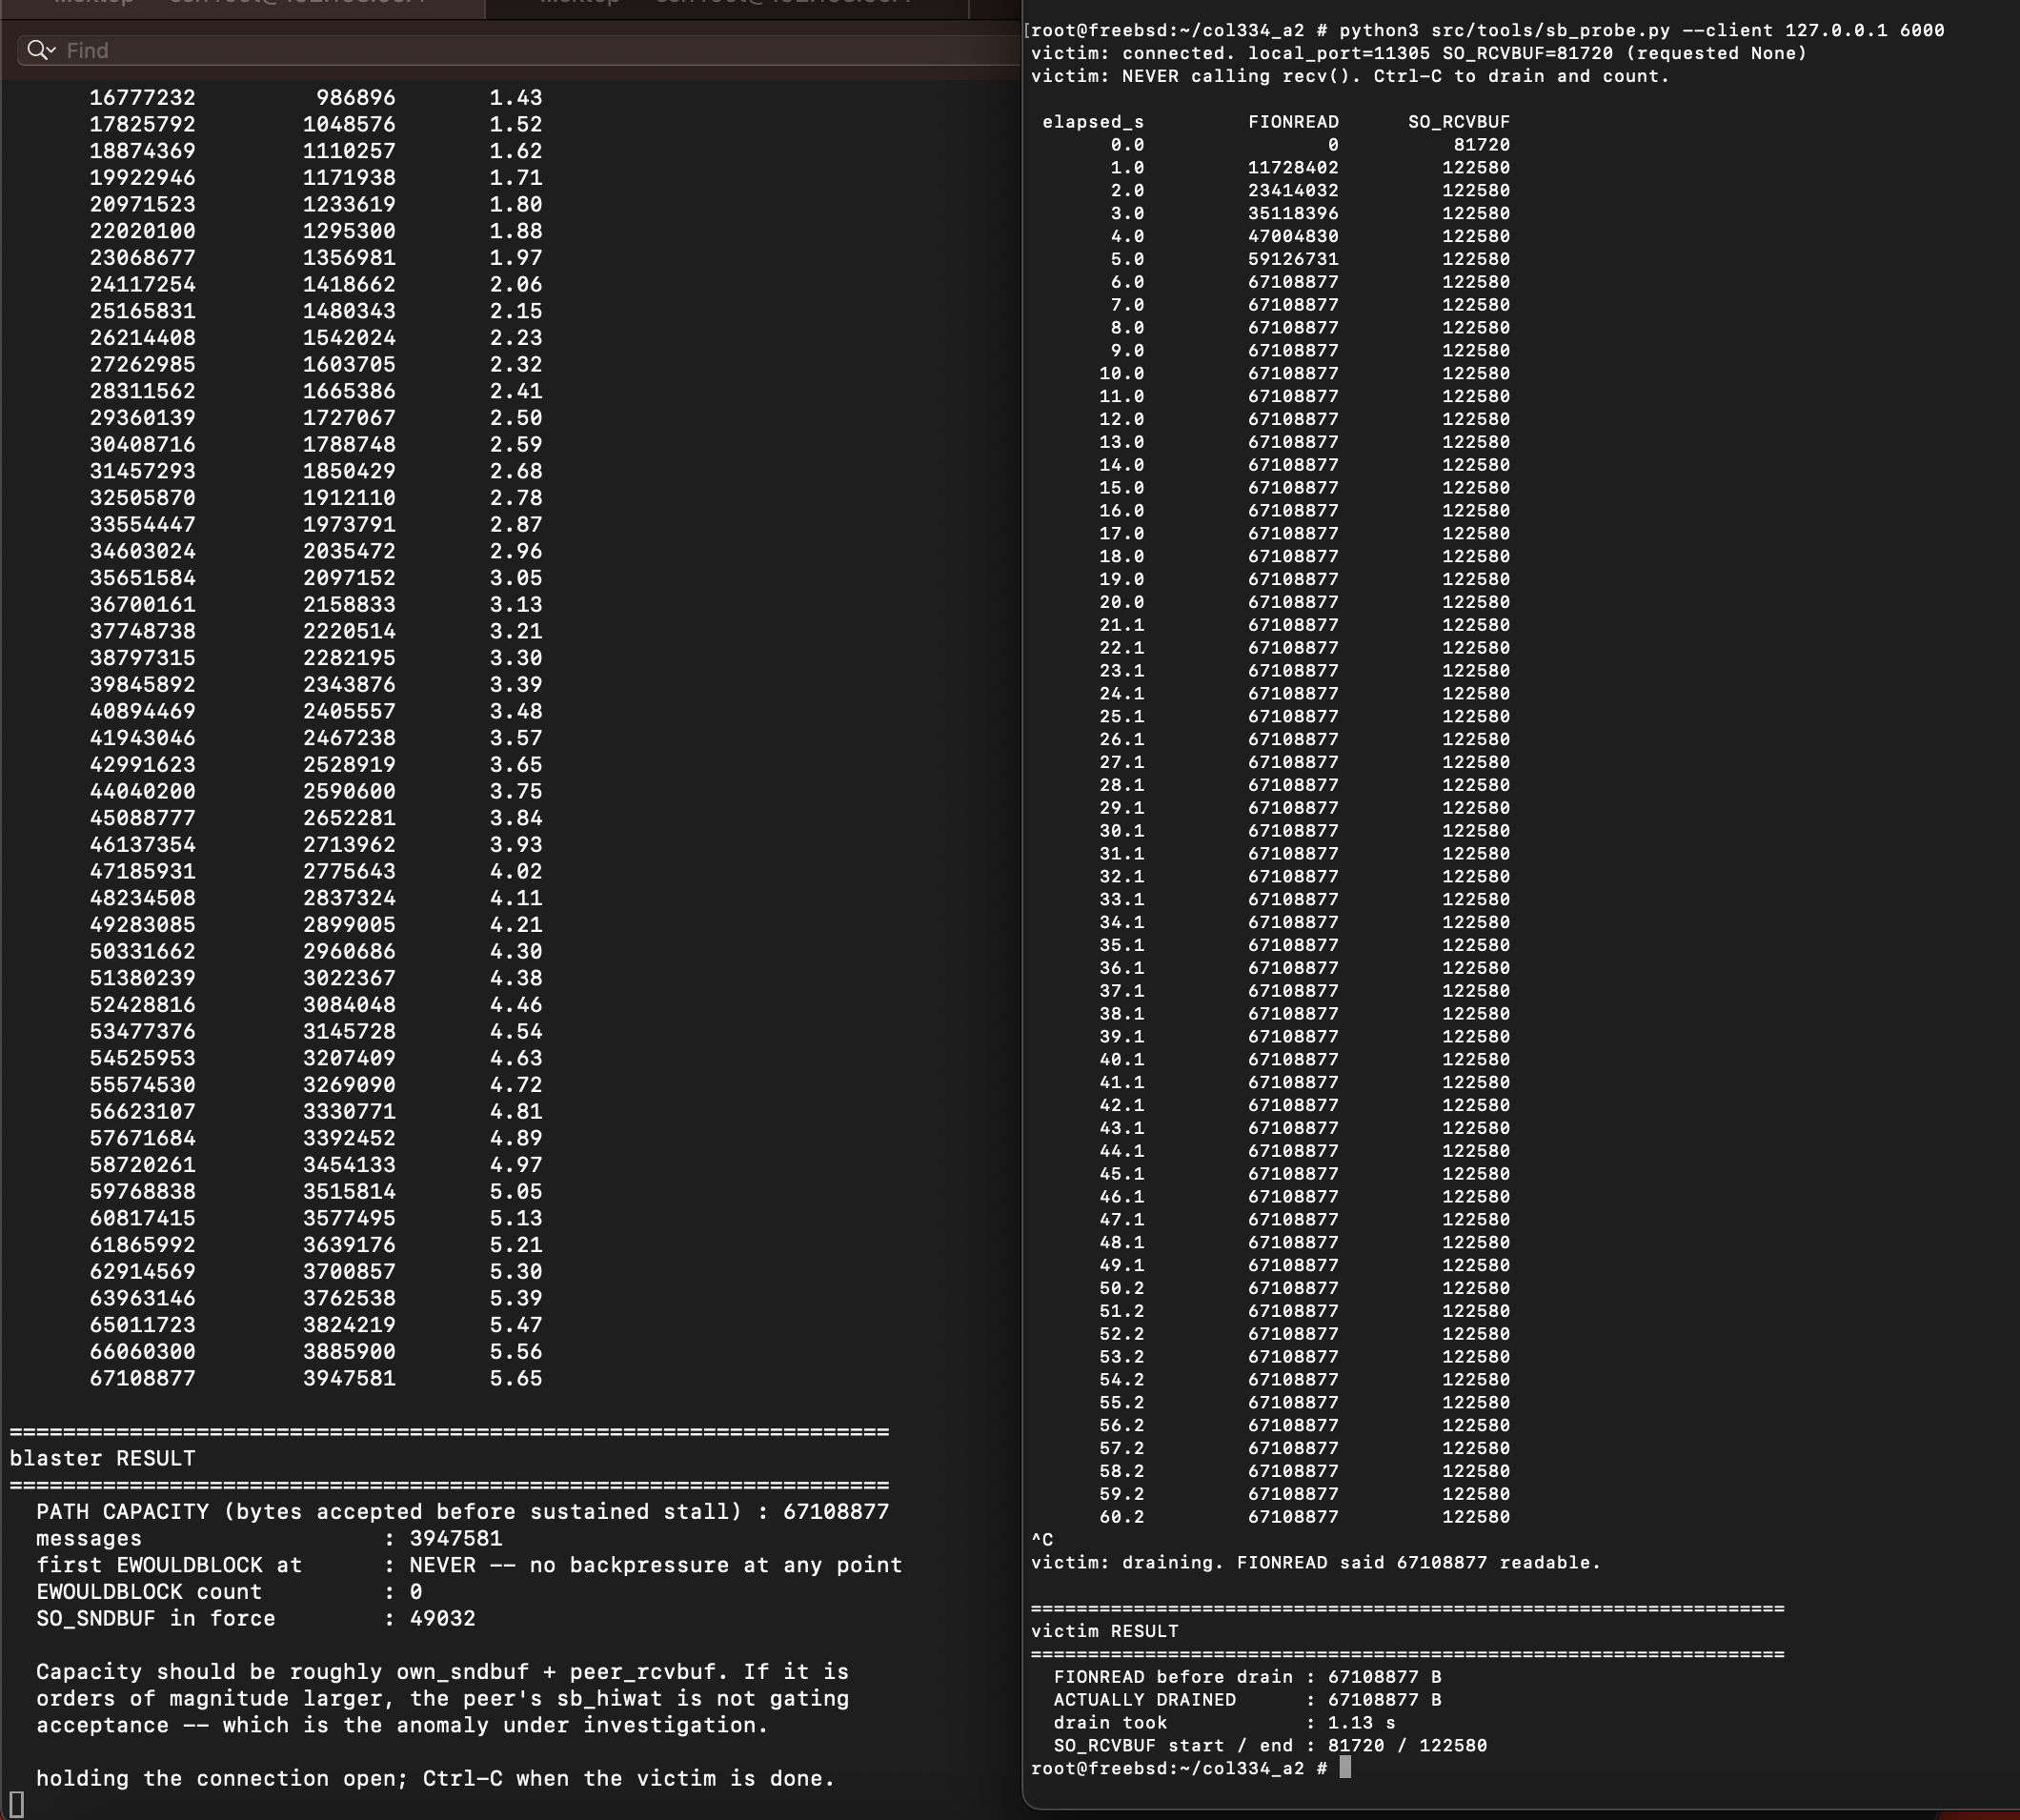
\includegraphics{screenshots/7b.png}\\
\emph{Figure 7b: \texttt{sb\_probe.py} diagnostic on FreeBSD: 67 MB
absorbed unread without stall (in contrast to Linux, which stalls at 17
KB).}

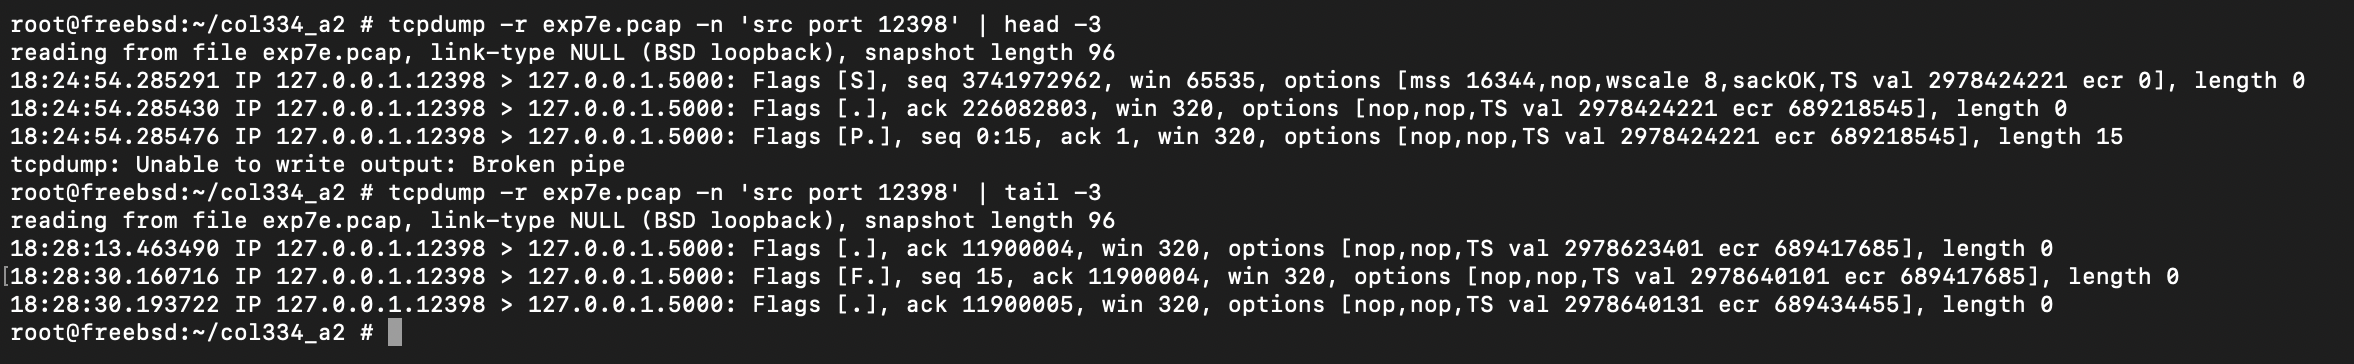
\includegraphics{screenshots/7c.png}\\
\emph{Figure 7c: Wire inspection on \texttt{exp7e.pcap} showing
subscriber maintaining a constant advertised window (\texttt{win\ 320} =
81,920 B) across 11.9 MB.}

\hypertarget{high-volume-verification-run-e}{%
\subsubsection{8.4 High-Volume Verification: Run
E}\label{high-volume-verification-run-e}}

To evaluate genuine backpressure handling under production-scale loads,
\texttt{exp7\_load.py} was executed with 700,000 matched order pairs
(stock sysctl settings):

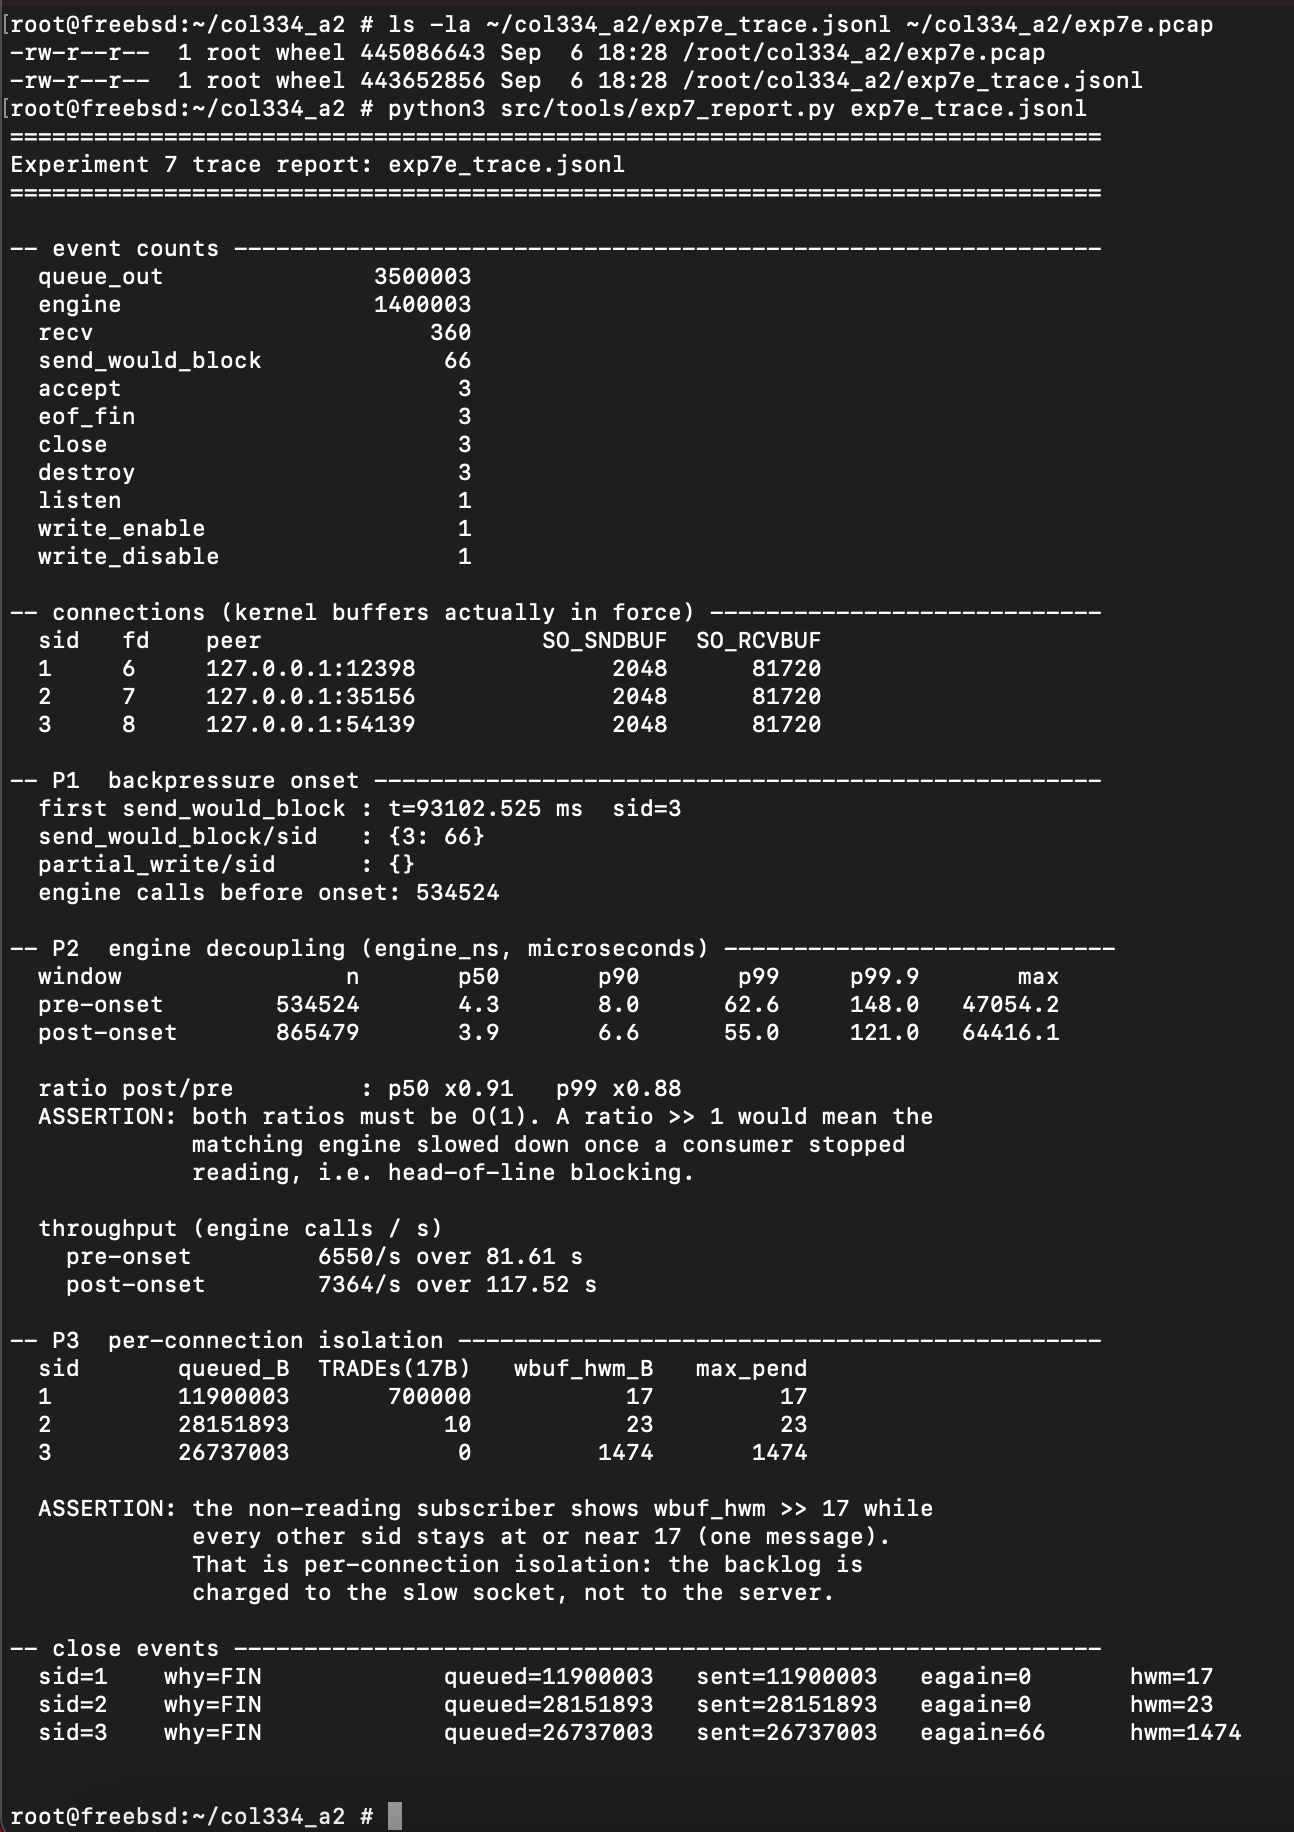
\includegraphics{screenshots/7d.png}\\
\emph{Figure 7d: \texttt{exp7\_report.py} output displaying backpressure
onset, per-session statistics, and engine latency.}

\textbf{Table 8: High-Volume Session Summary (Run E)}

\begin{longtable}[]{@{}
  >{\centering\arraybackslash}p{(\columnwidth - 8\tabcolsep) * \real{0.2000}}
  >{\centering\arraybackslash}p{(\columnwidth - 8\tabcolsep) * \real{0.2000}}
  >{\centering\arraybackslash}p{(\columnwidth - 8\tabcolsep) * \real{0.2000}}
  >{\centering\arraybackslash}p{(\columnwidth - 8\tabcolsep) * \real{0.2000}}
  >{\centering\arraybackslash}p{(\columnwidth - 8\tabcolsep) * \real{0.2000}}@{}}
\toprule\noalign{}
\begin{minipage}[b]{\linewidth}\centering
Session
\end{minipage} & \begin{minipage}[b]{\linewidth}\centering
Role
\end{minipage} & \begin{minipage}[b]{\linewidth}\centering
Total Queued
\end{minipage} & \begin{minipage}[b]{\linewidth}\centering
Peak Userspace Backlog (\texttt{wbuf\_hwm})
\end{minipage} & \begin{minipage}[b]{\linewidth}\centering
\texttt{EAGAIN} Events
\end{minipage} \\
\midrule\noalign{}
\endhead
\bottomrule\noalign{}
\endlastfoot
\texttt{sid=1} & Subscriber (Never reads) & 11,900,003 B & 17 B & 0 \\
\texttt{sid=2} & Buyer (Trader) & 28,151,893 B & 23 B & 0 \\
\texttt{sid=3} & Seller (Trader) & 26,737,003 B & \textbf{1,474 B} &
\textbf{66} \\
\end{longtable}

The 66 \texttt{EAGAIN} events occurred on \texttt{sid=3} due to
batch-write bursts. The server correctly responded by arming
\texttt{KQ\_FILTER\_WRITE}, buffering the excess in userspace, and
resuming writes without blocking.

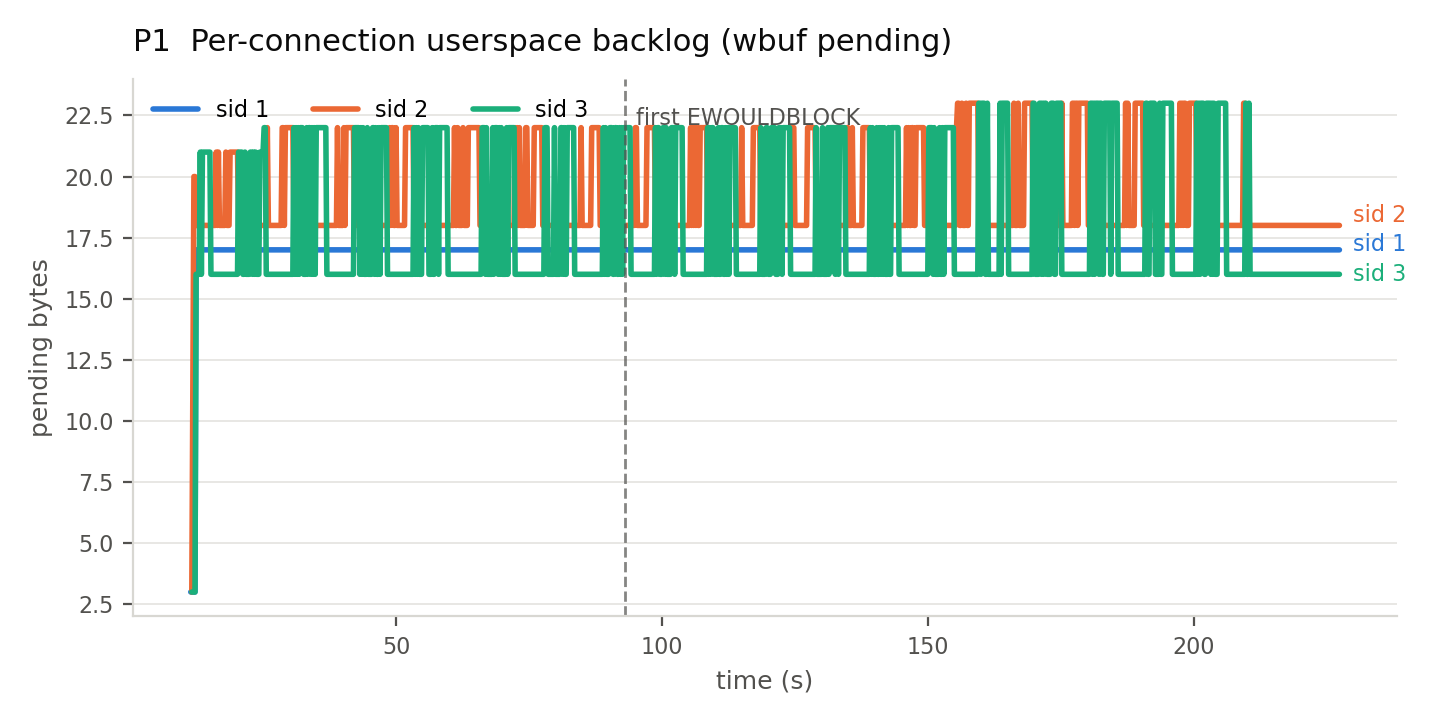
\includegraphics{figs/P1_pending.png}\\
\emph{Figure 7e: Per-connection userspace backlog over time, showing
transient buffering on \texttt{sid=3} with zero impact on other
sessions.}

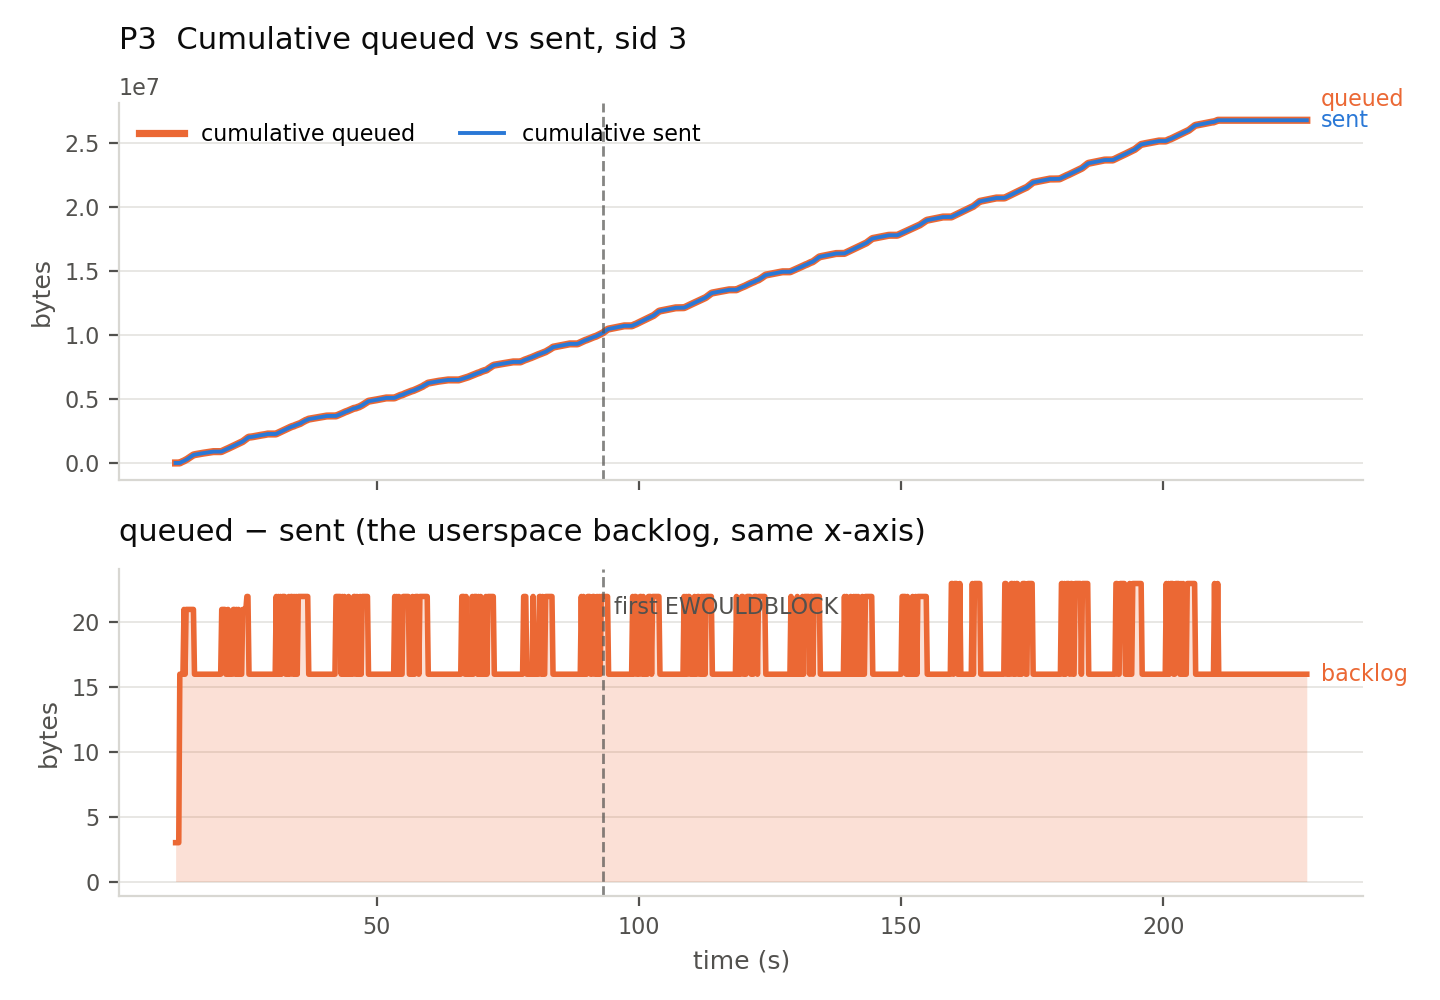
\includegraphics{figs/P3_queued_sent.png}\\
\emph{Figure 7f: Cumulative transmission volume vs.~transient backlog
delta for \texttt{sid=3}.}

\hypertarget{matching-engine-decoupling-proof}{%
\subsubsection{8.5 Matching Engine Decoupling
Proof}\label{matching-engine-decoupling-proof}}

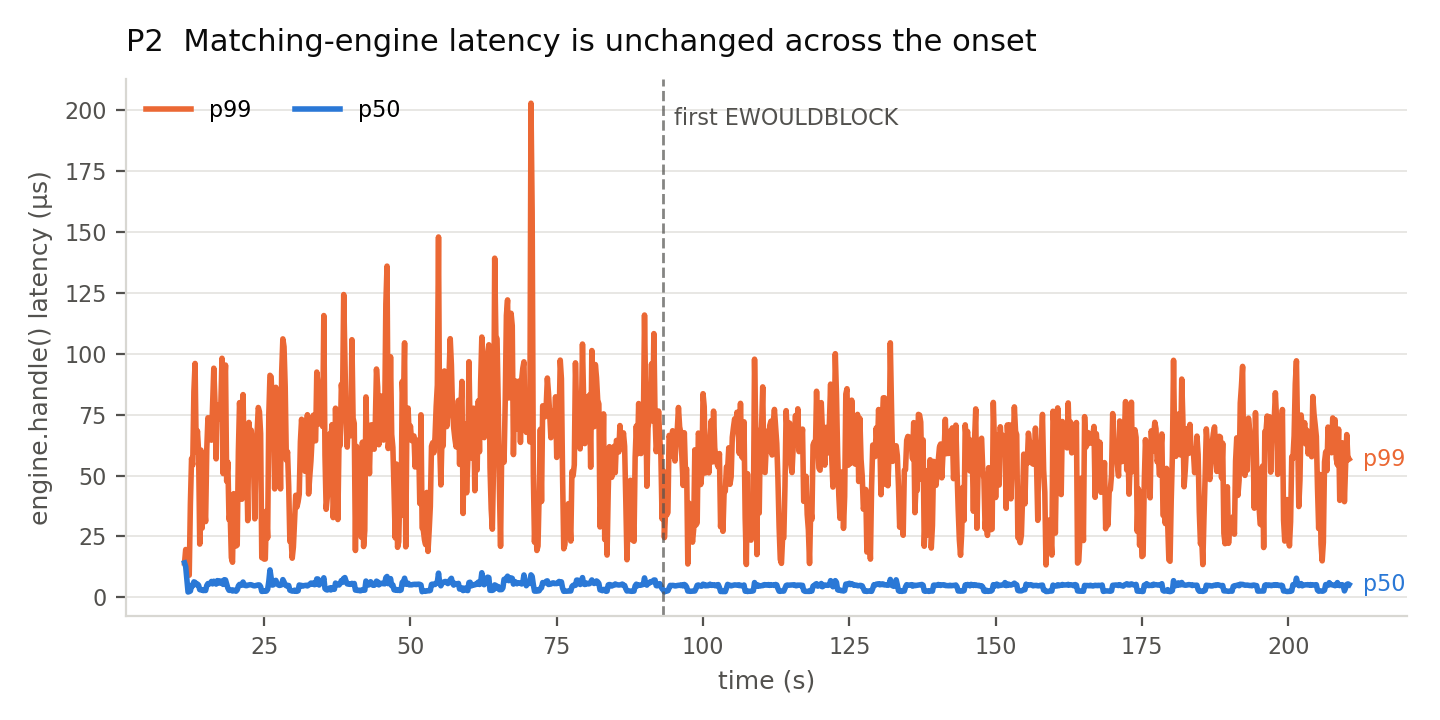
\includegraphics{figs/P2_engine.png}\\
\emph{Figure 7g: Matching engine execution latency distribution across
pre-onset and post-onset phases.}

\textbf{Table 9: Matching Engine Latency Distribution Across
Backpressure Onset}

\begin{longtable}[]{@{}
  >{\raggedright\arraybackslash}p{(\columnwidth - 12\tabcolsep) * \real{0.1176}}
  >{\centering\arraybackslash}p{(\columnwidth - 12\tabcolsep) * \real{0.1471}}
  >{\centering\arraybackslash}p{(\columnwidth - 12\tabcolsep) * \real{0.1471}}
  >{\centering\arraybackslash}p{(\columnwidth - 12\tabcolsep) * \real{0.1471}}
  >{\centering\arraybackslash}p{(\columnwidth - 12\tabcolsep) * \real{0.1471}}
  >{\centering\arraybackslash}p{(\columnwidth - 12\tabcolsep) * \real{0.1471}}
  >{\centering\arraybackslash}p{(\columnwidth - 12\tabcolsep) * \real{0.1471}}@{}}
\toprule\noalign{}
\begin{minipage}[b]{\linewidth}\raggedright
Window
\end{minipage} & \begin{minipage}[b]{\linewidth}\centering
Order Operations
\end{minipage} & \begin{minipage}[b]{\linewidth}\centering
p50 Latency
\end{minipage} & \begin{minipage}[b]{\linewidth}\centering
p90 Latency
\end{minipage} & \begin{minipage}[b]{\linewidth}\centering
p99 Latency
\end{minipage} & \begin{minipage}[b]{\linewidth}\centering
Max Latency
\end{minipage} & \begin{minipage}[b]{\linewidth}\centering
Throughput
\end{minipage} \\
\midrule\noalign{}
\endhead
\bottomrule\noalign{}
\endlastfoot
\textbf{Pre-Onset} & 534,524 & \(4.3\,\mu\text{s}\) &
\(8.0\,\mu\text{s}\) & \(62.6\,\mu\text{s}\) & \(47.0\,\text{ms}\) &
6,550 ops/s \\
\textbf{Post-Onset} & 865,479 & \textbf{\(3.9\,\mu\text{s}\)} &
\textbf{\(6.6\,\mu\text{s}\)} & \textbf{\(55.0\,\mu\text{s}\)} &
\(64.4\,\text{ms}\) & \textbf{7,364 ops/s} \\
\end{longtable}

Engine latency remained constant across the backpressure boundary (p50
ratio: 0.91, p99 ratio: 0.88), providing empirical proof that network
write stalls do not impede order processing.

\begin{center}\rule{0.5\linewidth}{0.5pt}\end{center}

\hypertarget{experiment-8-unexpected-client-disconnection}{%
\subsection{9. Experiment 8 --- Unexpected Client
Disconnection}\label{experiment-8-unexpected-client-disconnection}}

\hypertarget{technical-analysis-6}{%
\subsubsection{9.1 Technical Analysis}\label{technical-analysis-6}}

When a client process is terminated abruptly via \texttt{SIGKILL}, the
process is unable to execute user-space shutdown logic. However, the
operating system kernel reclaims all open file descriptors on process
death, transmitting an orderly \texttt{FIN} segment.

The Exchange Server detects client loss reactively upon the next event
loop iteration. Disconnection of one client must not interrupt active
trading between surviving participants. Furthermore, resting orders
submitted prior to termination must persist in the book and remain
eligible for execution (§2.6).

\hypertarget{investigation-methodology-tools-5}{%
\subsubsection{9.2 Investigation Methodology \&
Tools}\label{investigation-methodology-tools-5}}

\begin{Shaded}
\begin{Highlighting}[]
\ExtensionTok{tcpdump} \AttributeTok{{-}i}\NormalTok{ lo0 }\AttributeTok{{-}n} \AttributeTok{{-}s0} \AttributeTok{{-}w}\NormalTok{ exp8.pcap }\StringTok{\textquotesingle{}tcp port 5000\textquotesingle{}} \KeywordTok{\&}
\ExtensionTok{python3}\NormalTok{ experiment.py 8}
\ExtensionTok{tcpdump} \AttributeTok{{-}r}\NormalTok{ exp8.pcap }\AttributeTok{{-}n} \AttributeTok{{-}ttt} \AttributeTok{{-}S} \KeywordTok{|} \FunctionTok{grep} \OperatorTok{\textless{}}\NormalTok{killed\_port}\OperatorTok{\textgreater{}}
\end{Highlighting}
\end{Shaded}

\hypertarget{empirical-evidence-6}{%
\subsubsection{9.3 Empirical Evidence}\label{empirical-evidence-6}}

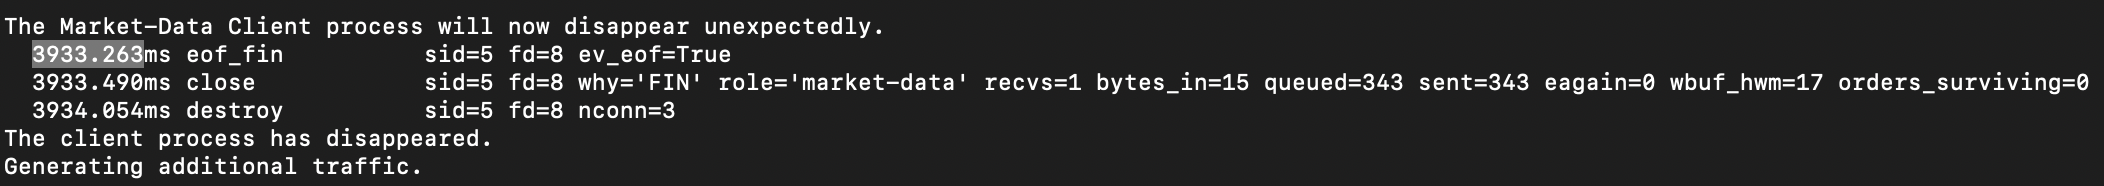
\includegraphics{screenshots/8a.png}\\
\emph{Figure 8a: Server logs verifying client termination detection,
session cleanup, and continued trade execution.}

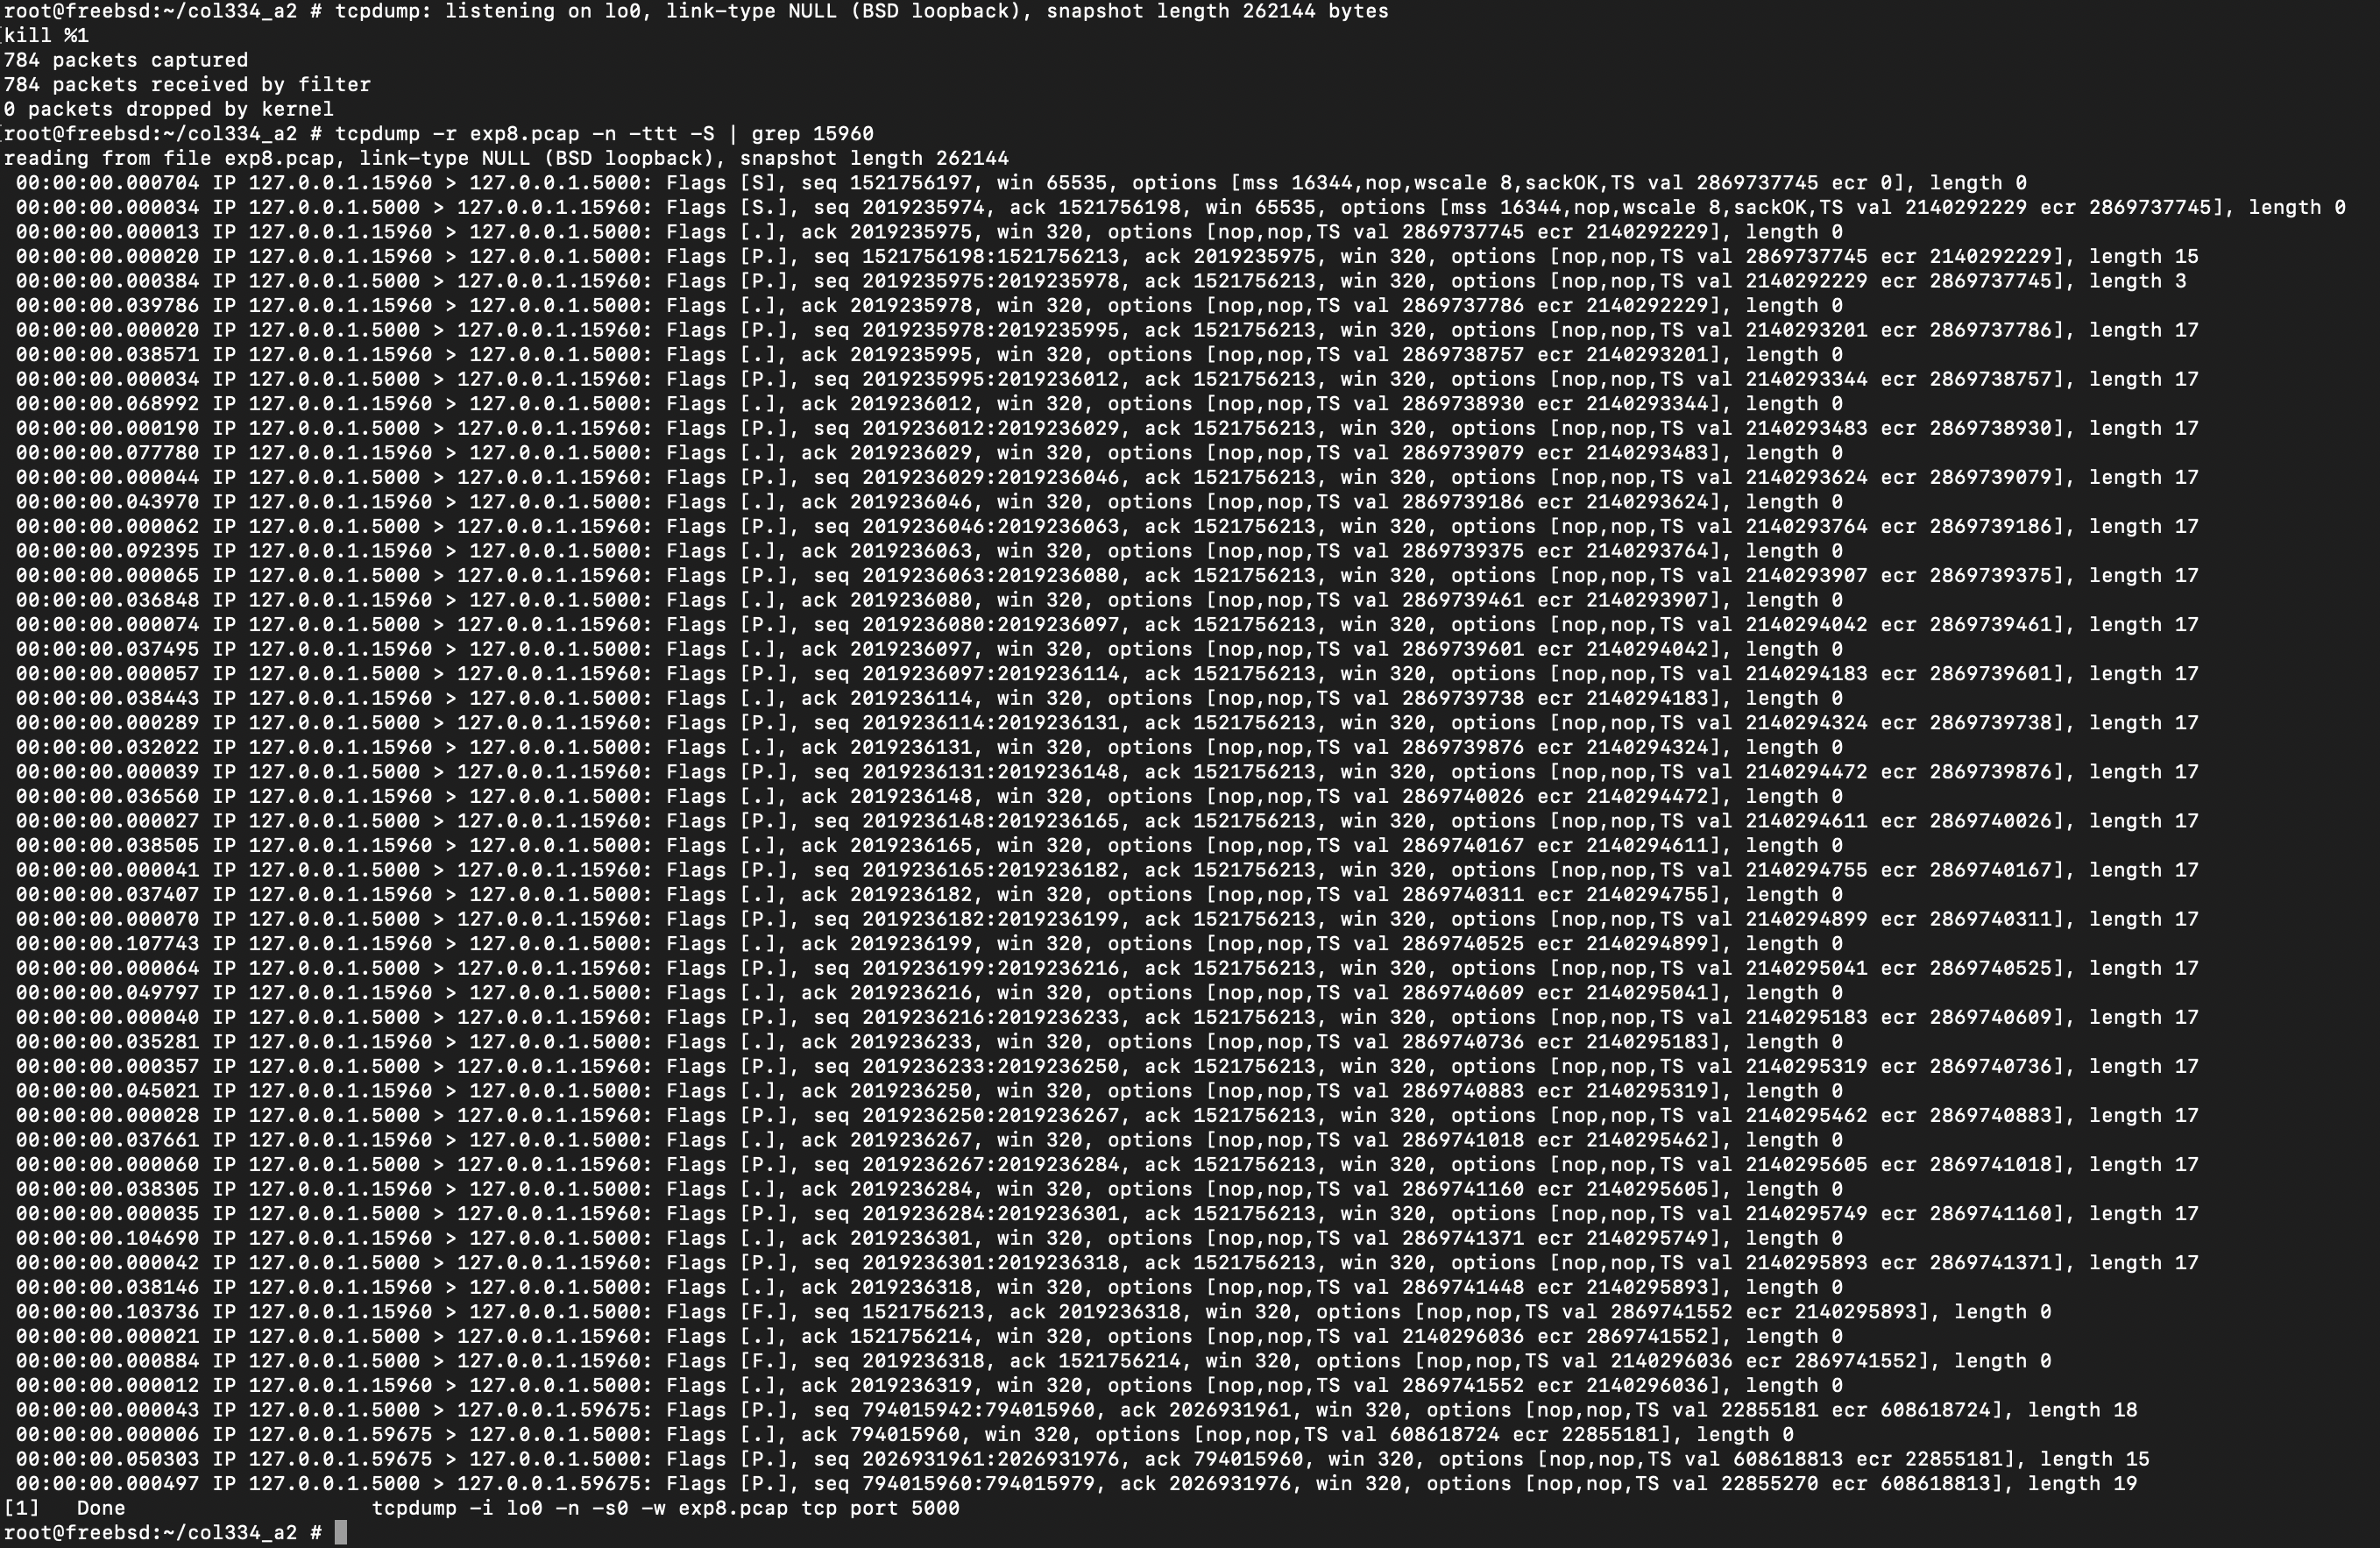
\includegraphics{screenshots/8b.png}\\
\emph{Figure 8b: Packet capture confirming kernel-issued FIN handshake
following \texttt{SIGKILL}.}

\textbf{Wire Event Chronology:}

\begin{verbatim}
15960 > 5000: Flags [.]  ack 1                (Last subscriber ACK)
15960 > 5000: Flags [F.] seq 1 ack 1          (Kernel-generated FIN on SIGKILL)
5000 > 15960: Flags [.]  ack 2                (Server ACK)
5000 > 15960: Flags [F.] seq 1 ack 2          (Server FIN teardown)
15960 > 5000: Flags [.]  ack 2                (Final ACK, teardown complete)
\end{verbatim}

\textbf{Table 10: Process Termination vs.~Order Survival Event Log}

\begin{longtable}[]{@{}
  >{\centering\arraybackslash}p{(\columnwidth - 6\tabcolsep) * \real{0.2941}}
  >{\raggedright\arraybackslash}p{(\columnwidth - 6\tabcolsep) * \real{0.2353}}
  >{\raggedright\arraybackslash}p{(\columnwidth - 6\tabcolsep) * \real{0.2353}}
  >{\raggedright\arraybackslash}p{(\columnwidth - 6\tabcolsep) * \real{0.2353}}@{}}
\toprule\noalign{}
\begin{minipage}[b]{\linewidth}\centering
Time (ms)
\end{minipage} & \begin{minipage}[b]{\linewidth}\raggedright
Component
\end{minipage} & \begin{minipage}[b]{\linewidth}\raggedright
Action / Observation
\end{minipage} & \begin{minipage}[b]{\linewidth}\raggedright
Architectural Significance
\end{minipage} \\
\midrule\noalign{}
\endhead
\bottomrule\noalign{}
\endlastfoot
3933.26 & Kernel / TCP & \texttt{SIGKILL} sent to client; kernel emits
\texttt{FIN} & Process death surfaces as normal EOF \\
3933.49 & Server Reactor & \texttt{eof\_fin} detected; \texttt{close()}
triggered & Descriptor closed cleanly, removed from \texttt{by\_sid} \\
3934.05 & Server Reactor & Descriptor destroyed (\texttt{nconn=3}) &
Surviving connections continue uninterrupted \\
4012.00 & Trading Engine & Subsequent BUY/SELL pairs submitted &
Matching engine executes subsequent trades normally \\
4012.10 & Market Data & Surviving subscriber receives \texttt{TRADE}
updates & Broadcast pipeline remains fully functional \\
\end{longtable}

\hypertarget{supplementary-proof-resting-order-survival-post-disconnect}{%
\subsubsection{9.4 Supplementary Proof: Resting Order Survival
Post-Disconnect}\label{supplementary-proof-resting-order-survival-post-disconnect}}

Because the harness in Experiment 8 terminates a Market-Data subscriber
(which holds no orders), a dedicated test verified the survival of
resting trader orders:

\begin{enumerate}
\def\labelenumi{\arabic{enumi}.}
\tightlist
\item
  Trader A connects (\texttt{sid=2}), places
  \texttt{BUY\ JNST\ 100\ 238} (order 0), and disconnects.
\item
  Trader B connects (\texttt{sid=3}), places
  \texttt{SELL\ JNST\ 60\ 238}.
\item
  Order 0 matches for 60 units. Trader B receives
  \texttt{SOLD\ JNST\ 60\ 238}, active subscribers receive
  \texttt{TRADE\ JNST\ 60\ 238}, and Trader A's private notification is
  safely dropped:
\end{enumerate}

\begin{verbatim}
close sid=2 why='FIN' role='trader' orders_surviving=1
engine trade match: BUY 0 vs SELL 1 -> 60 JNST @ 238
notify_dropped: target_sid=2 msg=b'BOUGHT JNST 60 238\n'
\end{verbatim}

\begin{center}\rule{0.5\linewidth}{0.5pt}\end{center}

\hypertarget{system-concurrency-protocol-verification}{%
\subsection{10. System Concurrency \& Protocol
Verification}\label{system-concurrency-protocol-verification}}

\hypertarget{handout-4.3-concurrency-verification-ge-10-clients}{%
\subsubsection{\texorpdfstring{10.1 Handout §4.3 Concurrency
Verification (\(\ge 10\)
Clients)}{10.1 Handout §4.3 Concurrency Verification (\textbackslash ge 10 Clients)}}\label{handout-4.3-concurrency-verification-ge-10-clients}}

Handout Section 4.3 mandates simultaneous support for at least 10 active
clients, including at least 2 Trader Clients and at least 4 Market-Data
Clients.

This requirement was validated using
\texttt{src/tools/gapd\_concurrency.sh}, which launches 4 concurrent
Trader Clients and 6 concurrent Market-Data Clients (10 total) against
an active server. All 10 connections established and operated
simultaneously without degradation:

\begin{verbatim}
$ sockstat -4 | grep :5000 | grep ESTABLISHED | wc -l
20    # 10 client endpoints + 10 server-side peer endpoints
\end{verbatim}

\hypertarget{outbound-and-inbound-message-coalescing}{%
\subsubsection{10.2 Outbound and Inbound Message
Coalescing}\label{outbound-and-inbound-message-coalescing}}

TCP stream framing was verified in both directions:

\begin{itemize}
\tightlist
\item
  \textbf{Inbound Coalescing:} Multiple complete commands transmitted in
  a single TCP segment
  (\texttt{LOGIN\ client\_1\textbackslash{}nBUY\ JNST\ 100\ 238\textbackslash{}n})
  are sequentially parsed and dispatched by \texttt{Framer.feed()}.
\item
  \textbf{Outbound Latency Optimization:} \texttt{queue\_out()} issues
  opportunistic flushes with \texttt{TCP\_NODELAY}. Under normal
  conditions, replies are dispatched immediately; when peer backpressure
  occurs, messages coalesce automatically in userspace \texttt{wbuf},
  optimizing throughput.
\end{itemize}

\hypertarget{protocol-error-vocabulary-errno-matrix}{%
\subsubsection{10.3 Protocol Error Vocabulary \& Errno
Matrix}\label{protocol-error-vocabulary-errno-matrix}}

The server handles errors strictly and uniformly across all interaction
paths:

\textbf{Table 11: Operating System Errno Mapping}

\begin{longtable}[]{@{}
  >{\centering\arraybackslash}p{(\columnwidth - 6\tabcolsep) * \real{0.2941}}
  >{\raggedright\arraybackslash}p{(\columnwidth - 6\tabcolsep) * \real{0.2353}}
  >{\raggedright\arraybackslash}p{(\columnwidth - 6\tabcolsep) * \real{0.2353}}
  >{\raggedright\arraybackslash}p{(\columnwidth - 6\tabcolsep) * \real{0.2353}}@{}}
\toprule\noalign{}
\begin{minipage}[b]{\linewidth}\centering
Errno
\end{minipage} & \begin{minipage}[b]{\linewidth}\raggedright
Symbol
\end{minipage} & \begin{minipage}[b]{\linewidth}\raggedright
System Event
\end{minipage} & \begin{minipage}[b]{\linewidth}\raggedright
Implementation Response
\end{minipage} \\
\midrule\noalign{}
\endhead
\bottomrule\noalign{}
\endlastfoot
\textbf{35} & \texttt{EAGAIN} / \texttt{EWOULDBLOCK} & Socket send
buffer full & Catch \texttt{BlockingIOError}, buffer in \texttt{wbuf},
arm \texttt{KQ\_FILTER\_WRITE}. \\
\textbf{54} & \texttt{ECONNRESET} & Peer abortive reset (\texttt{RST}) &
Detected via \texttt{ev.fflags=54}, mark dead, purge session. \\
\textbf{32} & \texttt{EPIPE} & Write to closed peer & Intercepted via
\texttt{BrokenPipeError}, close descriptor cleanly. \\
\textbf{60} & \texttt{ETIMEDOUT} & Peer dropped silently & Handled by OS
TCP keepalive / retransmit exhaustion. \\
\end{longtable}

\begin{center}\rule{0.5\linewidth}{0.5pt}\end{center}

\hypertarget{codebase-structure-reproduction-commands}{%
\subsection{11. Codebase Structure \& Reproduction
Commands}\label{codebase-structure-reproduction-commands}}

\hypertarget{source-code-architecture}{%
\subsubsection{11.1 Source Code
Architecture}\label{source-code-architecture}}

\begin{verbatim}
server/run-server           Executable launcher for Exchange Server
client/run-trader           Executable launcher for Trader Client
client/run-market-data      Executable launcher for Market-Data Client
src/server.py               Main kqueue reactor, buffer manager, and network I/O
src/engine.py               Order book, matching engine, and session management
src/protocol.py             Byte-level parsing, numerical validation, and error strings
src/framing.py              Stream framing and newline delimiter extraction
src/trader.py               Interactive/automated trader client (multiplexed stdin)
src/market_data.py          Interactive/automated market data client
tests/test_all.py           Offline verification suite (framing, engine, validation)
\end{verbatim}

\hypertarget{reproduction-commands}{%
\subsubsection{11.2 Reproduction Commands}\label{reproduction-commands}}

To run the automated experiment suite:

\begin{Shaded}
\begin{Highlighting}[]
\CommentTok{\# Ensure launchers have execute permissions}
\FunctionTok{chmod}\NormalTok{ +x server/run{-}server client/run{-}trader client/run{-}market{-}data}

\CommentTok{\# Execute experiments 1 through 8}
\ExtensionTok{python3}\NormalTok{ experiment.py 1}
\ExtensionTok{python3}\NormalTok{ experiment.py 2}
\ExtensionTok{python3}\NormalTok{ experiment.py 3}
\ExtensionTok{python3}\NormalTok{ experiment.py 4}
\ExtensionTok{python3}\NormalTok{ experiment.py 5}
\ExtensionTok{python3}\NormalTok{ experiment.py 6}
\ExtensionTok{python3}\NormalTok{ experiment.py 7}
\ExtensionTok{python3}\NormalTok{ experiment.py 8}

\CommentTok{\# Run the 10{-}client concurrency test (§4.3)}
\FunctionTok{sh}\NormalTok{ src/tools/gapd\_concurrency.sh 127.0.0.1 5000}
\end{Highlighting}
\end{Shaded}

\begin{center}\rule{0.5\linewidth}{0.5pt}\end{center}

\hypertarget{edge-case-verification}{%
\subsection{12. Edge-Case Verification}\label{edge-case-verification}}

Additional terminal-based checks were performed against the framing,
protocol, matching, session-management, and socket write paths. These
checks supplemented the numbered experiments and did not require any
changes to the implementation.

\begin{itemize}
\tightlist
\item
  \textbf{TCP framing and incomplete input:} Commands split across
  multiple reads were reconstructed correctly, while several commands in
  one read were processed individually. A connection ending midway
  through a command did not execute the incomplete command.
\item
  \textbf{Session and role handling:} Duplicate usernames were rejected,
  usernames became available again after disconnection, unauthenticated
  trading commands were rejected, and Market-Data clients could not place
  orders.
\item
  \textbf{Numeric validation:} Zero, negative, malformed, and out-of-range
  quantities, prices, and order identifiers produced the corresponding
  protocol errors instead of entering the matching engine.
\item
  \textbf{Cancellation behavior:} Cancellation was verified for partially
  filled orders, repeated cancellation, unknown order identifiers, fully
  executed orders, and attempts made by a trader who did not own the
  order.
\item
  \textbf{Matching behavior:} Partial fills preserved the correct
  remaining quantity, one incoming order could fill against multiple
  resting orders, and equal-price orders were matched in arrival order.
\item
  \textbf{Disconnection cleanup:} Outstanding orders remained available
  for matching after their trader disconnected. Private notifications to
  departed traders were dropped safely, subscribed clients still received
  trade updates, and disconnected Market-Data clients were removed from
  later broadcasts.
\item
  \textbf{Backpressure and graceful termination:} A non-reading peer
  accumulated buffered output without blocking service to other clients.
  Once it resumed reading, the backlog drained. On \texttt{QUIT}, queued
  replies were sent before the connection closed, and commands following
  \texttt{QUIT} in the same batch were ignored.
\end{itemize}

All checks produced the expected protocol state and output.


\end{document}
